\chapter{\chapiiiname}
\label{chapter3}



\section*{Abstract}
% Add captivating abstract
This work has converged on using conductive particle elastomer composites (CPECs) as the electroactive base for creating improved sensor-actuator devices, due to their superior qualities outlined in the Literature Review. Understanding the dynamic characteristics of a CPEC is critical for using the material in dynamic sensor and actuator devices. Although the fabrication of a CPEC can be simple, the characterisation and optimisation of such a material for soft robotic applications can require complex models and display non-linear time-dependent behaviour. In this work we uncover several repeatable mathematical relationships seen within the material concerning dynamic time series behaviour between tensile strain, stress, and resistance data. 

First a linear quasi-static model is generated to give a simple formula for estimating strain given a resistance input for a steady state system. Then the time-dependent and dynamic phenomena of the CPEC material were explored. Analogously to fitting stress relaxation to a two-unit generalised Maxwell mechanical model, this work has fitted the resistive relaxation seen after a strain step input to a three-unit generalised Maxwell model. A non-linear relationship was found between resistive and stress relaxations, which disproves the hypothesis that the stress relaxation is directly related to the resistive relaxation. For a strain falling edge signal, a positive correlation was found between increased strain-rate and the resistance peak seen in the tensile specimens. Similarly a positive correlation was found between the pre-strain amplitude and the resistance peak generated, for a strain falling edge signal. We have demonstrated a technique to reduce apparent resistance measurement drift in resistance experiments by using a switched AC current source instead of DC.

All of the behaviours determined in this work set a foundation for understanding the viscoelastic electromechanical nature of a CPEC for further development of the material in more complex sensor and actuator systems. Future work aims to generate a non-linear inverse model to more accurately determine the strain of the CPEC material given a resistance input. Analysis will also be extended to not just the composite resistance but the resistivity to give more generalisable relationships. With this inverse model the CPEC material would be suited to a plethora of biomedical and agricultural applications which require delicate and non-toxic sensing systems.



\section{Introduction}
\label{sec:ch3-intro}
% Why does this chapter matter? What is the link to soft robotics and artificial skin/muscle?
% - Conductive particle elastomer composites are attractive for soft robotics because...
As discussed in the Literature Review chapter, conductive particle elastomer composites are desirable for soft sensor and actuator applications for a variety of reasons. However, it is crucial to understand the electromechanical behaviour of these composites if we wish to create complex control systems with such materials. Although conductive particle elastomer composites (CPECs) are simple in concept, consisting of dispersed particles through an elastomer matrix, the electromechanical behaviour is not well understood on a macro or micro-scale. This chapter will focuses on only tensile stress characterisation and modelling of the specimen. Compressive characterisation and modelling is covered in the subsequent chapters. This work endeavours to understand the material behaviours of carbon black silicone rubber composites on a macro-scale to help create improved inverse models so that the material can be used more accurately for stress/strain sensors. 
%\section{Stress and resistive relaxation For Carbon Nanoparticle Silicone Rubber Composite Large-Strain Sensors}
%\label{sec:Stress and resistive relaxation}
%\textit{From a conference paper presented at IDETC-MESA 2021}


\subsection{Background}
Carbon nanoparticle-silicone elastomer composites are stretchable conductive materials with diverse applications such as, highly elastic strain sensors \cite{Lacasse2010,Spahr2017,Kim2018}, dielectric elastomer actuators \cite{Henke2018,Liu2009} and electromyography electrodes \cite{Carpi2010,Kim2018,Mouri2019}. Understanding the dynamic resistive relaxation characteristics of carbon black (CB) silicone rubber (SR) elastomer composites would improve performance in fields which require high efficiency of space, power and accuracy, such as the devices used in biomedical and aerospace fields. Unlike many common strain gauges, CBSR composites can have strains of over 300\% without yielding \cite{Wang2010} depending on the type of SR and CB used and the method of fabrication. This strain and the strain used in this work is higher than commonly used constantan strain gauges, which typically have a maximum strain of $\pm 3$\% \cite{VishayPG2018}, with traditional metal alloy based strain gauges often having significant plastic deformation after less than $10^4$ cycles \cite{VishayPG2018} at this 3\% strain.


Some characteristics of CBSR composites which make it suitable for strain sensors include that, the material is relatively inexpensive, readily available, non-toxic, bio-compatible, and can have a high gauge factor. Other alternative composite conductive particles, such as carbon nanotubes (CNTs) \cite{Maddipatla2017,Wang2013} and metallic particles \cite{Quinsaat2015,Racles2021}, have been seen to be more carcinogenic than CB alternatives \cite{Fukushima2018,Ferdous2020,Rausch2004}. The fabrication of CBSR composites requires a degree of optimisation to ensure that the carbon particles are adequately dispersed to ensure high conductivity and high yield strength of the material. More importantly the homogeneous dispersion of CB particles means improved repeatability of experimental results and more accurate models for the eventual applications of CBSR composites. A comprehensive model of how the resistivity changes with strain has not yet been developed. 

While previous work from our research group \cite{Giffney2017,Devaraj2018} has focused on the response to quasi-static and low-strain-rate behaviour, these materials show dynamic effects where a significant resistance strain-rate relationship is present. The main characterisation investigated in this work for CBSR sensing involves understanding the relationship between the mechanical stress relaxation, electrical resistive relaxation and strain in time. A difference in time constants between the stress and resistive relaxations have been noted before in literature \cite{Kost1994,Wang2013,Maddipatla2017,Wang2004}, but never accurately modelled with the physical theory explained. Mersch et al. \cite{Mersch2020} have classified several transient `shoulder' events and their related deformation events, compressive, tensile, and bending. These transient peaks have been observed by several researchers using the similar CBSR materials, however there is no conclusive mathematical model relating these transient peaks to strain in time. An understanding of this resistive relaxation and other transient phenomena would mean an accurate model could be made to predict the relationship between stress, strain and resistance within a CBSR composite. 

Determining a stress-strain-resistance model would also allow us to understand the limitations of using this composite in sensing and actuation applications, so that the material can be used simultaneously as an actuation excitation electrode and a strain sensor. Understanding these characteristics may give rise to new applications of the composites material, for example, if the resistive relaxation properties of the material were known, it could be used as a mechanically activated timing device. An oscillatory flexible dynamic circuit has been demonstrated when mimicking the motion of a caterpillar as shown by Henke et al. \cite{Henke2018}, where the resistive relaxation modelling is be useful for more accurate electrical circuit dynamics. The theory behind mechanical stress relaxation is widely known and has been modelled using a variety of mathematical models \cite{Fung1993} depending on the material modelled. 

It is known that silicone rubber composites are viscoelastic materials and clearly exhibit the three traits of a viscolelastic material \cite{Fung1993}: stress relaxation, strain creep, and stress-strain hysteresis. Stress relaxation is an effect observed when a step input of strain is applied to a material and there is a transient stress decay response which converges to a steady state value. A commonly used model for viscoelasticty is the generalised Maxwell body model of order $n$ shown in Figure \ref{fig:Maxwell_general}.
\begin{figure}[H]
	\centering
	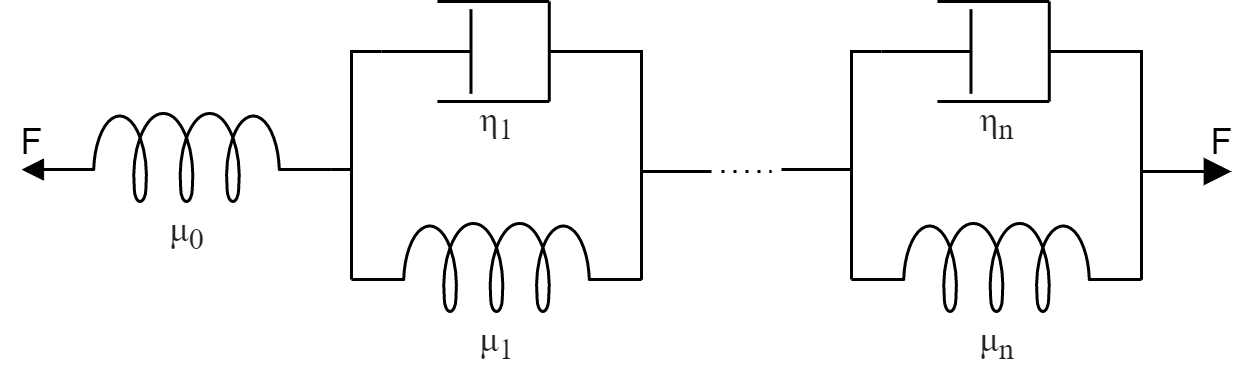
\includegraphics[width=0.7\linewidth]{Figures/Generlised_Maxwell_body.png}
	\caption{Mechanical spring dashpot diagram of the generalised Maxwell body model adapted from Fung et al. \cite{Fung1993}}
	\label{fig:Maxwell_general}
\end{figure}
Where $F$ is the force applied to the material, and $\mu$ and $\eta$ values represent the spring and damping component constants, respectively. The stress relaxation function for this model is found in Equation \ref{eqn:Maxwell_general}, for, $n$, serial repeating units. 
\begin{equation}
	G(t) = a_0 + \sum^n_{i=1} a_i \cdot e^{-t/\tau_i}
	\label{eqn:Maxwell_general} 
\end{equation}
Where $a_0$, $a_i$ are the magnitudes of relaxation and $\tau_i$ are the relaxation decay time constant components. All of the constants $a_0$, $a_i$, and $\tau_i$ are functions of $\eta$ and $\mu$. 

We initially assume that there is a relationship between the stress relaxation and resistive relaxation of the material. However, the generalised model can easily over-fit the data, if $n$ is too high. To mitigate over-fitting, a generalised model with the minimum amount of repeating units while maintaining a high $R^2$ is used.

Few mathematical models describing the viscoelastic-resistance relationship have been formulated. Laaraibi et al. \cite{Laaraibi2023} developed a time-invariant model which uses a relaxation parameter to account for the viscoleastic effect. Mersch et al. \cite{Mersch2020} developed a model using transverse and longitudinal viscoelastic parameters to model a similar CBSR material. Both models show promise towards creating a more comprehensive physical model. However, the both models aren't tested for a randomised range of input strain signals.
%\begin{equation}
%	R_{dynamic} = R_0 \cdot (1-\varepsilon) \cdot e^{-\theta \cdot \varepsilon}
%	\label{eqn:Anas-res-strain}
%\end{equation}
%\begin{equation}
%	R = K1_S \cdot (e^{K2_S \cdot \varepsilon_{Long}}+e^{K2_S \cdot \varepsilon_{Tra}}) + K1_F \cdot (e^{K2_F \cdot F_{Long}}+e^{K2_F \cdot F_{Tra}})
%	\label{eqn:Mersch-res-strain}
%\end{equation}



\section{Methods}
The core experimental part of this chapter will be described from composite fabrication through to simultaneous strain tensile tests and resistance measurements. This is followed by the analysis data for resistance-strain phenomena, to quantitatively match the phenomena these to black-box and viscoelastic models.


\subsection{Composite Fabrication}
The CBSR composite was composed of Vulcan XC-72 CB powder (Fuel Cell Store, Bryan, USA) and two part Pt cured Dragon Skin 10 NV SR (SmoothOn, Macungie, USA). The CB powder has an average particle size of 50 nm and typical bulk density of 96 kg/m$^3$. This grade of SR was chosen due to the following characteristics low elastic modulus, $E$, of 186 kPa tensile strength, $\sigma_Y$, of 2.75 MPa, and a low mixed viscosity, $\eta$, of 6,000 cps \cite{SmoothOn2021}. This $E$ value is within the range of human skin tissue and the low $\eta$ facilitates material processing in potential future applications with additive manufacturing.

The volume resistivity of pure CB powder itself is between $10^{-1}$ and $10^2 \mathrm{\Omega \cdot cm}$ depending on how densely the particles are packed and the purity of the CB \cite{Spahr2017}. The ability of a CB matrix embedded within a highly insulative SR substrate to become conductive is determined mainly by the dispersion of the CB particles, and the tunneling that occurs between conductive CB and insulative SR bodies within the material volume \cite{Spahr2017,Wang2013}. The composite being created must be highly conductive without compromising the elastic modulus and yield strength of the material. From percolation theory observed in literature \cite{Spahr2017} there is a threshold volume percentage of CB required to ensure that conductivity is maintained with certainty throughout the composite volume within the linear volume resistivity region. The percolation threshold for composite used in this work was difficult to predict due to the unknown configurations of agglomerations and dispersion of CB particles within the composite material. Empirically it was found that a CB volume percentage of 7.5\% or greater meant the composite material had a resistivity of less than 3.5 $\mathrm{k\Omega \cdot cm}$ consistently with the fabrication method used.

The first fabrication step was to mix the CB nano-powder with part A of the liquid SR using a KK-50S planetary mixer (Kurabo, Osaka, Japan). A mixing function was used with specific rotational velocities and times for each axis, which was well suited towards de-aeration and viscous particle mixing. The composite mixture was then mixed with the cross-linker part B of the liquid SR using the same planetary mixing function to ensure adequate dispersion of the CB particles throughout the SR volume.
\begin{figure}[H]
	\centering
	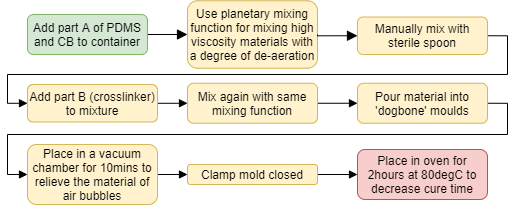
\includegraphics[width=0.8\linewidth]{Figures/specimenPrepFlowDiagram (1).png}
	\caption{The steps involved in creating the CBSR composite material}
	\label{fig:CBSR_flow_diagram}
\end{figure}
For the fabrication of the CBSR specimens, a standard dog-bone shaped mould was developed for the mixed CBSR to cure in, based on ASTM standard D412 \cite{ASTM2020}. Before the mould was clamped shut the composite filled mould was immediately placed in a vacuum chamber for ten minutes to de-aerate the still liquid, curing CBSR mixture. The specimen was placed in a lab oven at a temperature of 80 $^{\circ}$C for a two hours to accelerate curing. It has been shown that an increase in curing temperature for two part SR increases elastic moduli and decreases yield strength \cite{Johnston2014, Wu2005}.


\subsection{Material Imaging}
% This section will contain data gathered about the internal structure of the CBSR material. Including: Optical microscope, SEM, Raman spectroscopy, SAXS.
% Why is this section important? Ideally we would have an image of the percolated structure and how the particles move when deformed. However it is an arudous process to see nanometer scale structures using SEM or TEM and also run in-situ strain testing. Also the particles and agglomerates range from 50nm to ~5um in size, which means the largest particles can be seen with Raman and 50nm cannot be seen clearly by any method.
% What is the contribution towards research? Show some kind of patterning and agglomeration size??
% If we can find any form of fractal patterning at a micro-scale we could then imply that the fractal patterning exists at a nano-scale???Check-microscope,raman uscopy, and SEM for evidence of this!
To determine how the microstructure may effect the macro-behaviour observed in the following electro-mechanical testing of the material, three optical imaging methods were used, including optical microscopy, scanning electron microscopy (SEM), and Raman spectroscopy. 
% ... and small angle x-ray scattering (SAXS). 

The initial step was to observe the fabricated CBSR composite specimen using a stereoscopic microscope to view the internal structure of the CBSR composite specimens as shown in Figure \ref{fig:CBSR_8p_uscope_scalpel_frac}.
\begin{figure}[H]
	\centering
	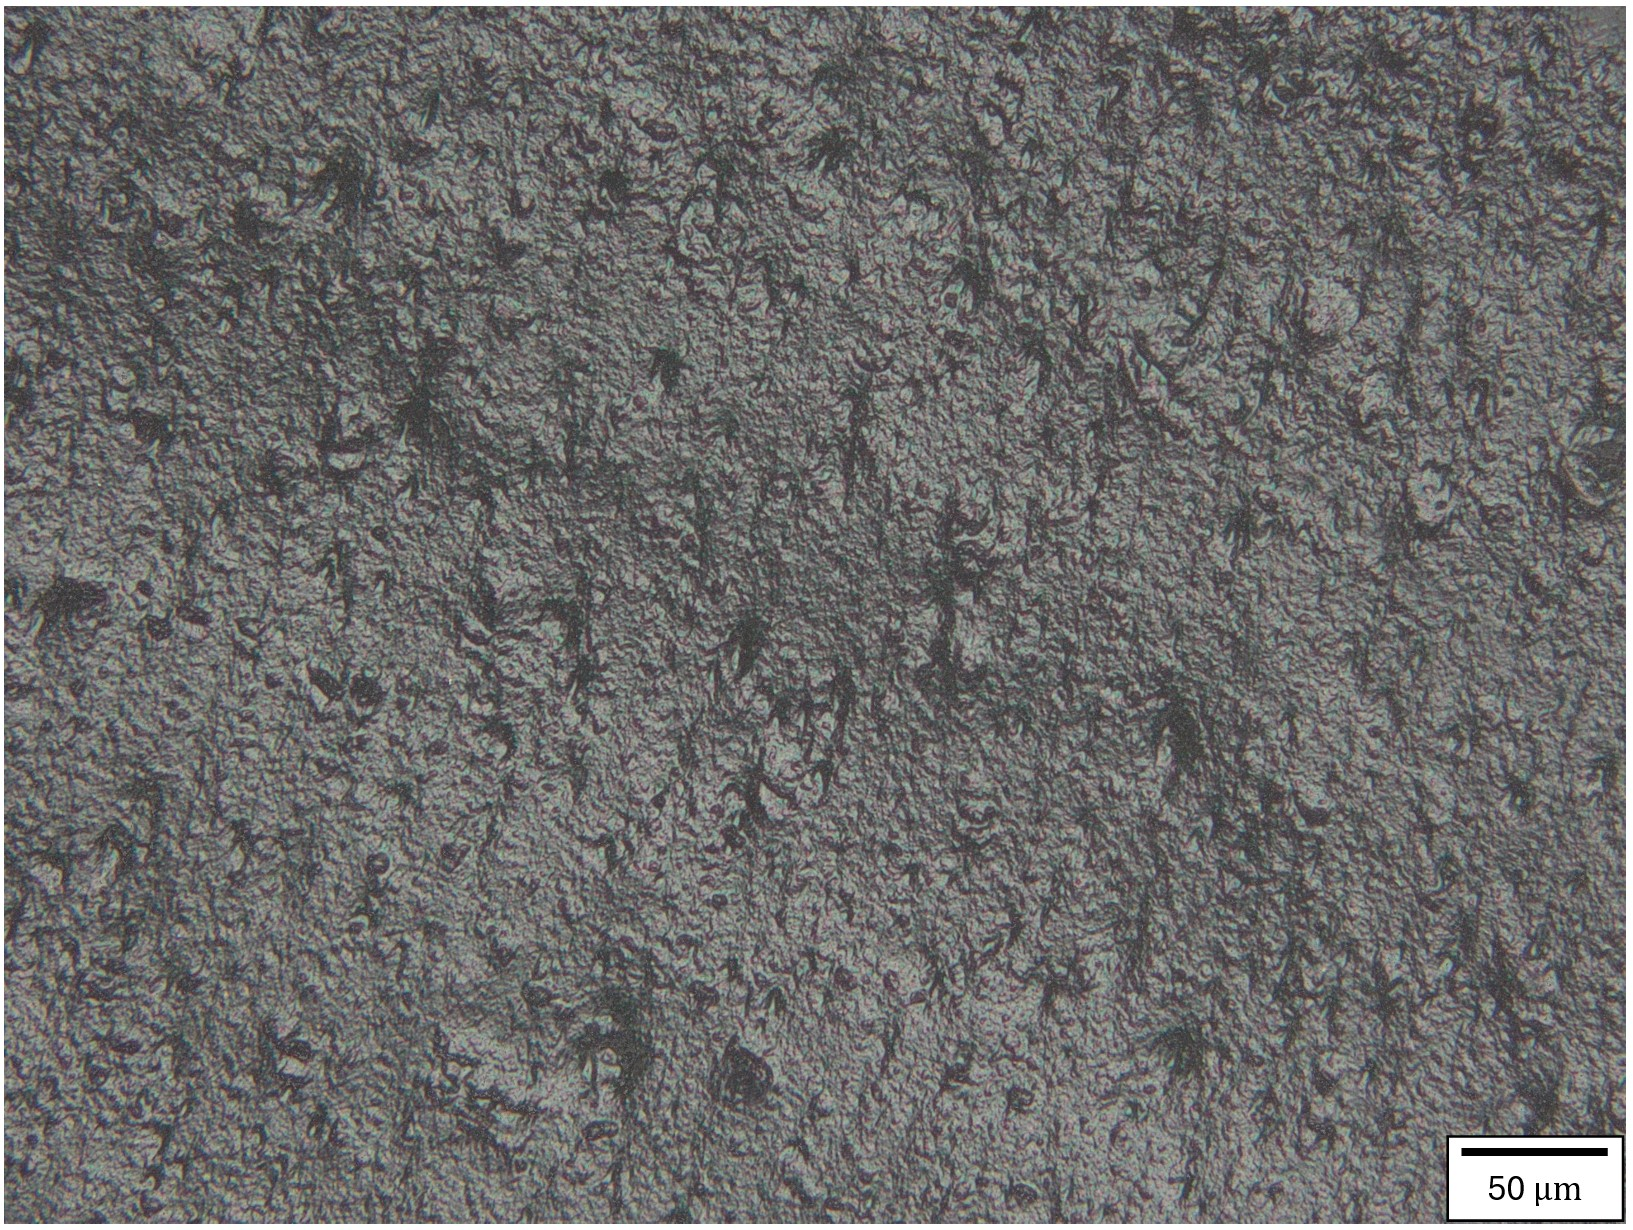
\includegraphics[width=0.4\linewidth]{Figures/scpl_cut_loc1_20x_CBSR_wt8.jpg}
	\hspace{0.5cm}
	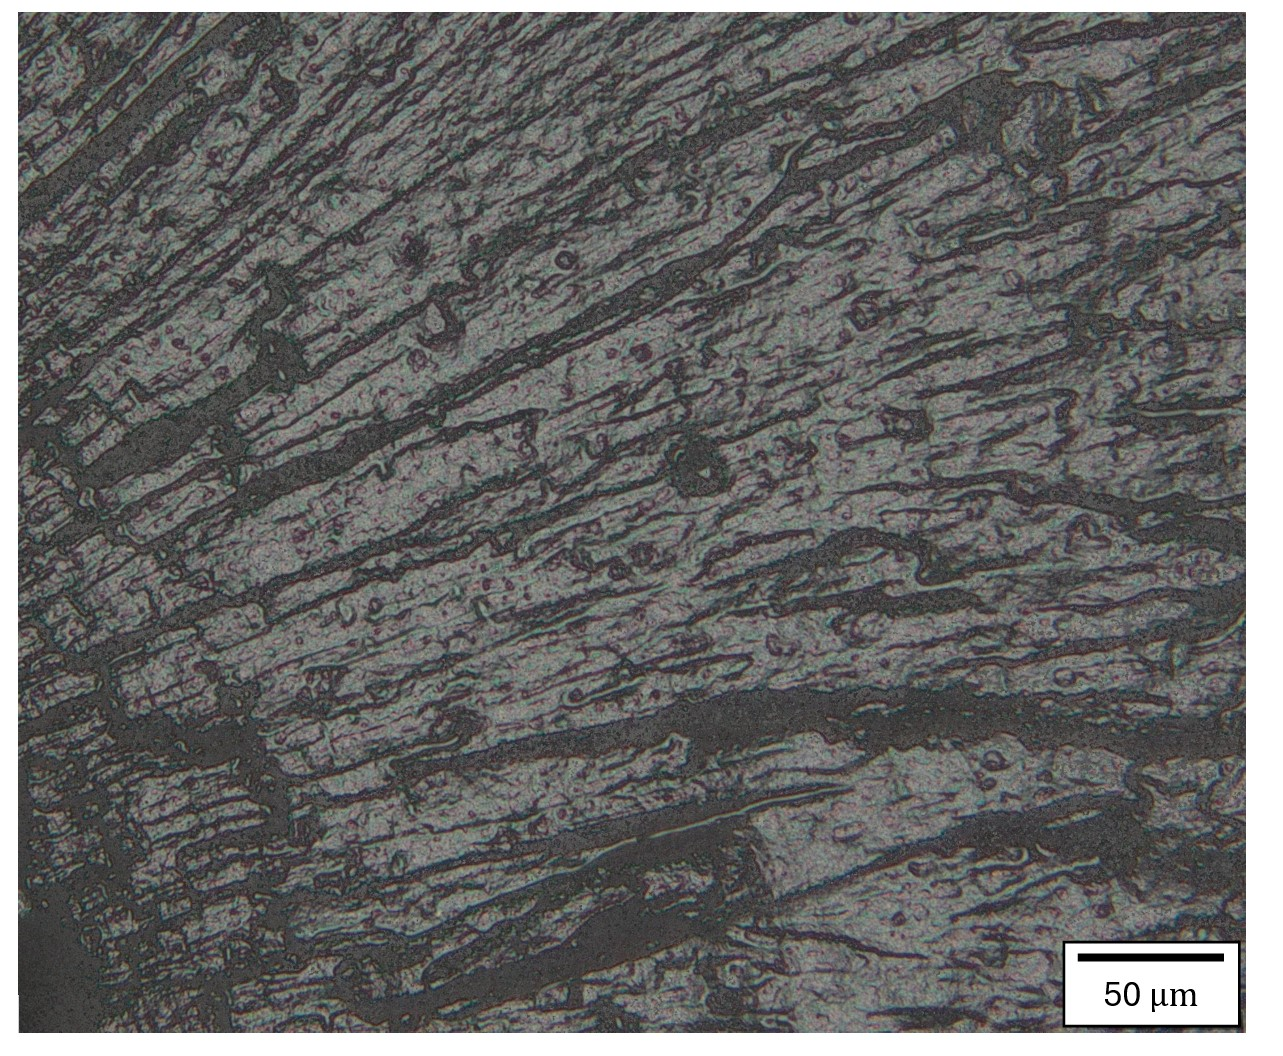
\includegraphics[width=0.37\linewidth]{Figures/br_frac_loc2_20x_CBSR_8wt.jpg}
	\caption{Microscope images at x20 magnification of a CBSR specimens with cross-sections made by; Left: Cutting with a scalpel. Right: Inducing an embrittlement fracture.}
	\label{fig:CBSR_8p_uscope_scalpel_frac}
\end{figure}
It is known in literature that preparing flat planar surfaces through elastomer composites for micro- and nano-scopic imaging is non-trivial \cite{Luo2005}. Due to the silicone material elasticity and a low embrittlement point of -60 to -70 $\degree$C , traditional polymer composite specimen machining methods cannot be used if a flat surface is desired. Because of the lack of water content in the CBSR composite traditional biological specimen preparations methods are also not feasible. 

% Could have trialled many more... e.g. LASER and water jet, but these may chemically alter and contaminate the specimen respectively.
Two methods were trialled to prepare the cross-sectional surface of the specimen for imaging, a scalpel cut and an induced embrittlement fracture. The scalpel cut was completed at room temperature conditions aligned vertically with the specimen. The induced embrittlement fracture used required extreme cooling by pouring liquid nitrogen over the specimen for 2 minutes, then snapping the specimen in two.

The induced embrittlement fracture shown in Figure \ref{fig:CBSR_8p_uscope_scalpel_frac} shows a very rough surface finish due to the many localised stress concentrations formed around voids and CB particles in the composite, and the non-crystallinity of the elastomer. The scalpel incision method showed an improved surface finish with a low amplitude undulating surface finish.

To observe smaller features such as voids and CB particle dispersion within the CBSR specimen the Apreo 2S FEG-SEM (Thermo Fisher Scientific, Waltham, USA) was used. Initially the CB particles were imaged validating their nominal primary particle size and displaying the agglomerated structure as shown in Figure \ref{fig:SEM_CB_SR}. The nominal particle size was found to be 48 $\pm$ 20 nm randomly sampling and averaging over 30 particles observed via SEM images. The top surface edge of the CBSR specimens were imaged to highlight the difference in surface roughnesses. Finally the dispersion of the CB particles was attempted, however due to surface charging of the relatively highly insulative silicone matrix the image resolution was limited as shown in \ref{fig:SEM_CB_SR}. 
\begin{figure}[H]
	\centering
    \begin{minipage}[t]{\textwidth}
		\centering
		\subfloat[][]{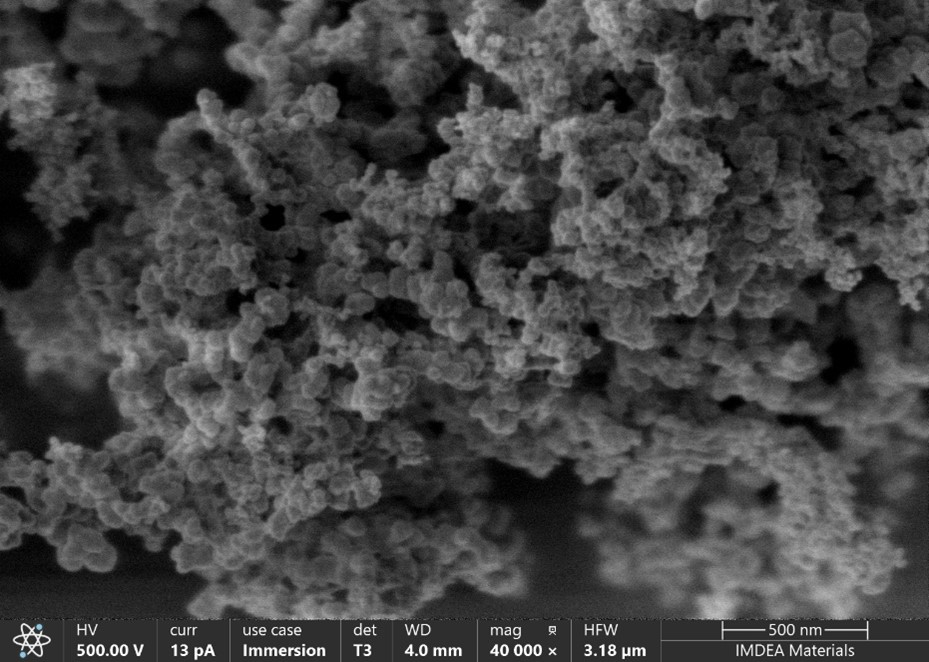
\includegraphics[width=0.5\textwidth]{Figures/CB_agglom_SEM.jpg}\label{subfig:SEM_CB}}
		\hspace{0.4cm}
		\subfloat[][]{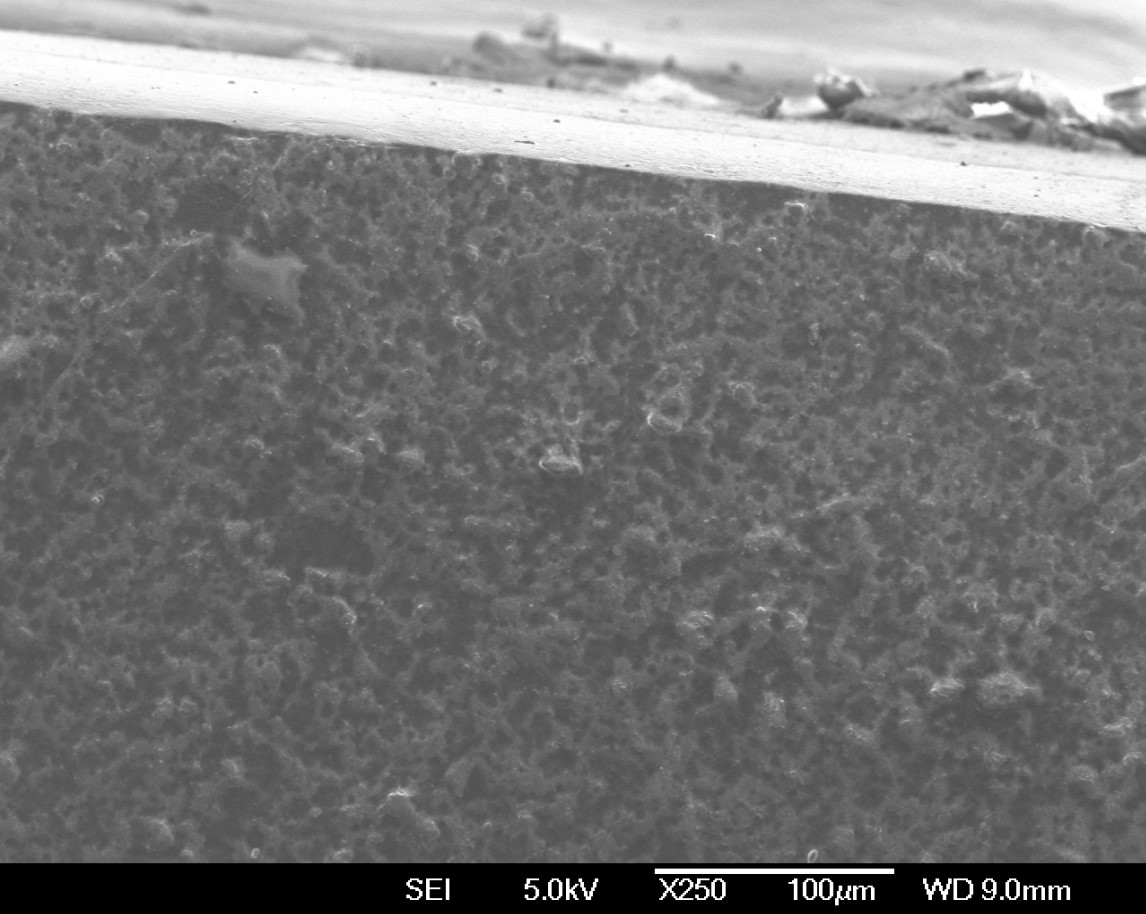
\includegraphics[width=0.45\textwidth]{Figures/CBSR_8wt_gold-coated-num15-x250-site-1-top.jpg}\label{subfig:SEM_CBSR_edge}}
	\end{minipage}
    \begin{minipage}[t]{\textwidth}
		\centering
		\vspace{0.4cm}
		\subfloat[][]{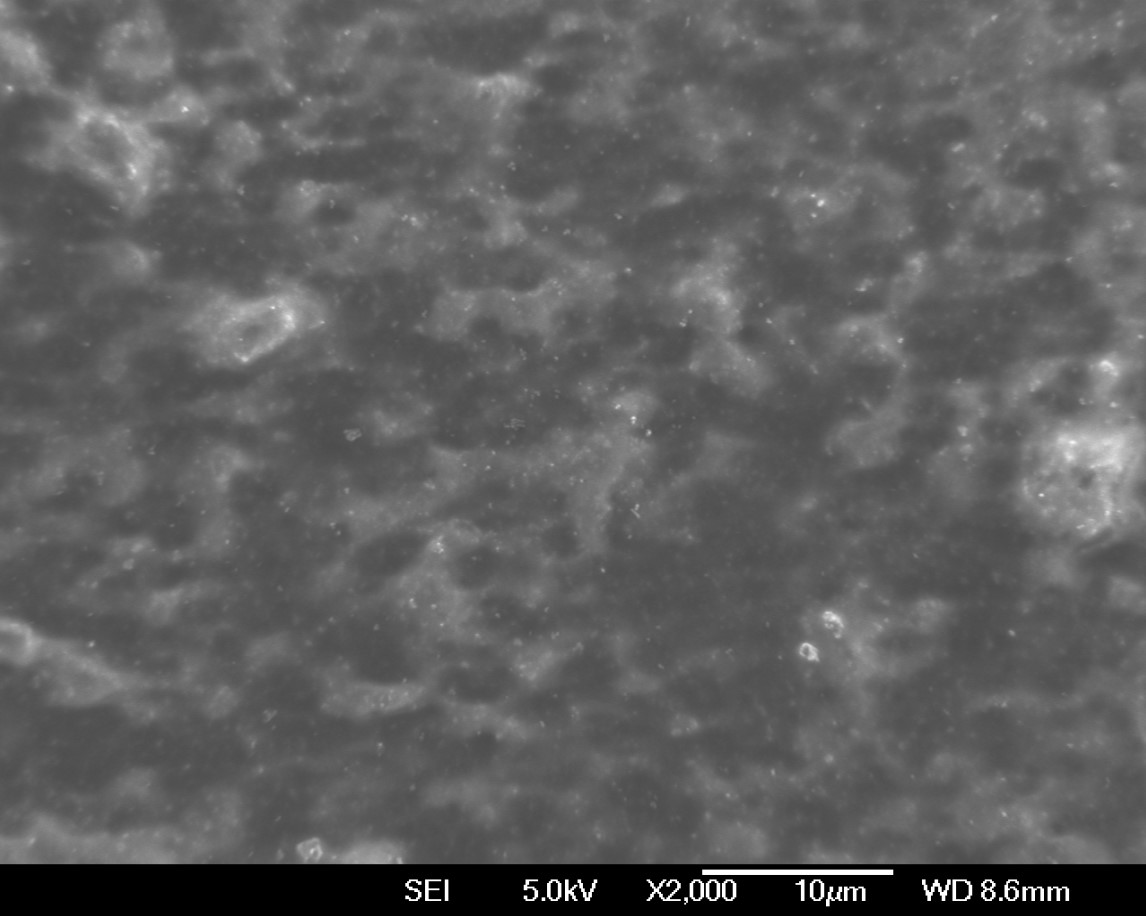
\includegraphics[width=0.45\textwidth]{Figures/CBSR_8wt_gold-coated-num10-x2000-site-1-top.jpg}\label{subfig:SEM_CBSR}}
	\end{minipage}
	\caption{SEM images of; (A): CB agglomerated particles $\times$40,000. (B): CBSR cross-section top surface edge site 1 $\times$250. (C): CBSR cross-section site 1 $\times$2000.}
	\label{fig:SEM_CB_SR}
\end{figure}
When measuring CBSR specimen for bulk electrical properties a reliable electrical connection to the material's conductive matrix is necessary. Obtaining high conductivity connection between the measurement electrodes and the material volume was investigated. The surface of the cured CBSR specimen is smooth and has proven highly insulative upon measurement, indicating that there is a thin insulative silicone film around the edges of the specimen as shown in Figure \ref{subfig:SEM_CBSR_edge}. This surface insulation film existed in each side of the specimen, potentially indicating that the viscosity of the SR matrix is high enough to prevent the CB nanoparticles from settling on the bottom surface of the mould used. The white dots shown in Figure \ref{subfig:SEM_CBSR} represent carbon particles throughout the SR matrix. Resolution was limited due to the insulative SR matrix charging from the electron beam. This is resolution discrepancy is apparent when comparing to the more conductive CB particles in Figure \ref{subfig:SEM_CB}.

To determine the presence and dispersion of CB particles on the surface of the CBSR specimens a inVia confocal Raman microscope (Renishaw, Wotton-under-Edge, United Kingdom) was used. A 532 nm laser with a was used in the Raman microscope. Several surface and cross-sectional images were taken showing a considerable difference in the CB-SR ratio as shown in Figure \ref{fig:Raman_CB_SR}. The prominent 1350 $cm^{-1}$ and 1600 $cm^{-1}$ intensity peaks indicate the presence of CB and the prominent 490 $cm^{-1}$, 2906 $cm^{-1}$, and 2965 $cm^{-1}$ peaks indicate the presence of SR \cite{Pawlyta2015,RamanLife2024}. 
\begin{figure}[H]
	\centering
    \begin{minipage}[t]{.49\textwidth}
    	\centering
    	\vspace{1cm}
		\subfloat[][]{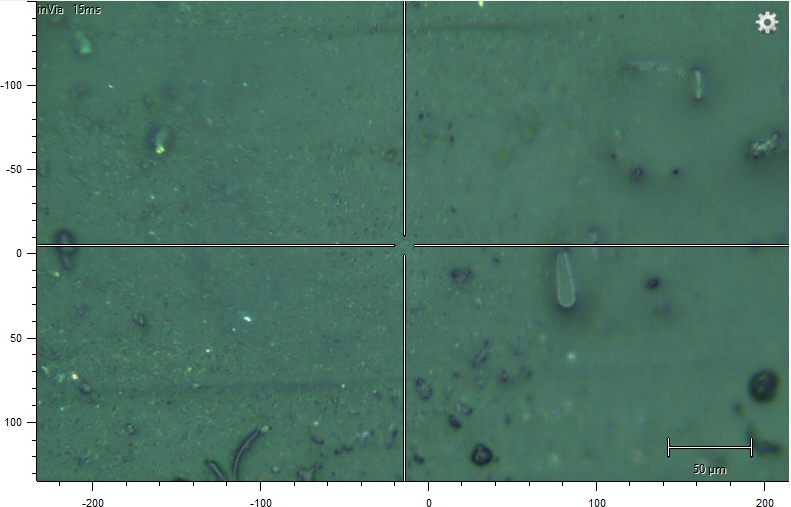
\includegraphics[width=0.85\textwidth]{Figures/Raman_still_9CBSR_50x_loc5.jpg}\label{subfig:raman_still}}
		\vfill
		\vspace{0.3cm}
		\subfloat[][]{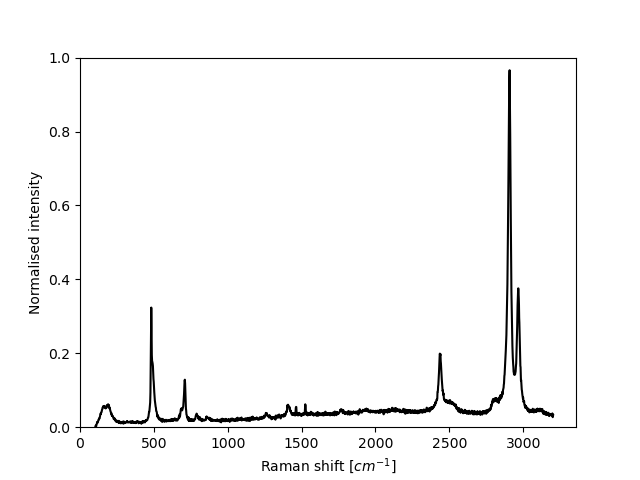
\includegraphics[width=0.95\textwidth]{Figures/Raman_0CBSR_10s_LP1_AC1_50x_loc1.png}\label{subfig:raman_0CB}
		}
	\end{minipage}
    \begin{minipage}[t]{.49\textwidth}
    	\centering
		\subfloat[][]{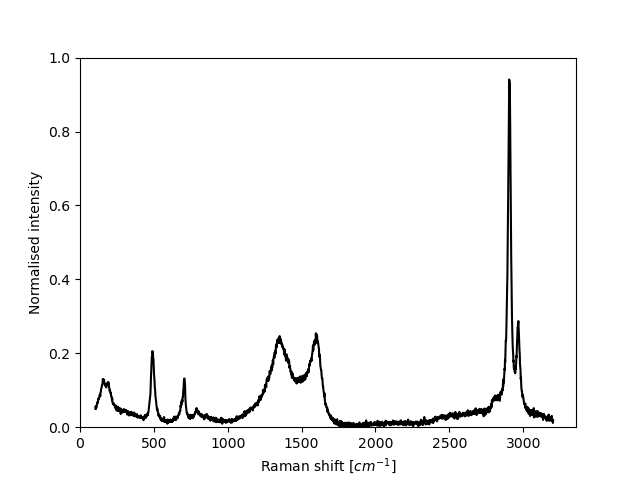
\includegraphics[width=0.95\textwidth]{Figures/Raman_8CBSR_10s_LP5_AC1_20x_loc1.png}\label{subfig:raman_8CB_surface}}
		\vfill
		\subfloat[][]{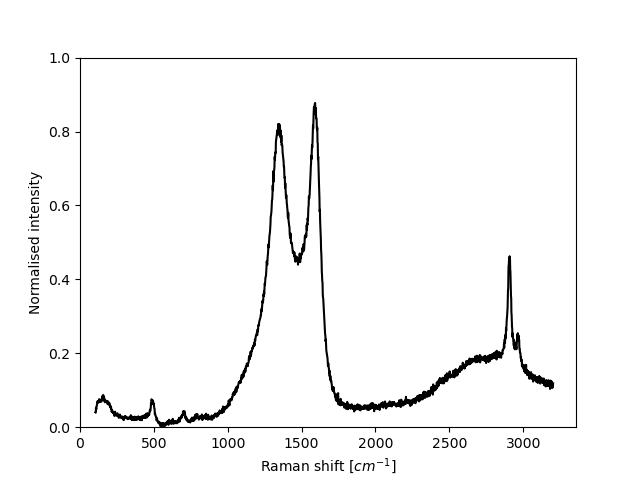
\includegraphics[width=0.95\textwidth]{Figures/Raman_cut8CBSR_10s_LP5_AC1_20x_loc1.png}\label{subfig:raman_8CB_cut}}
	\end{minipage}
%	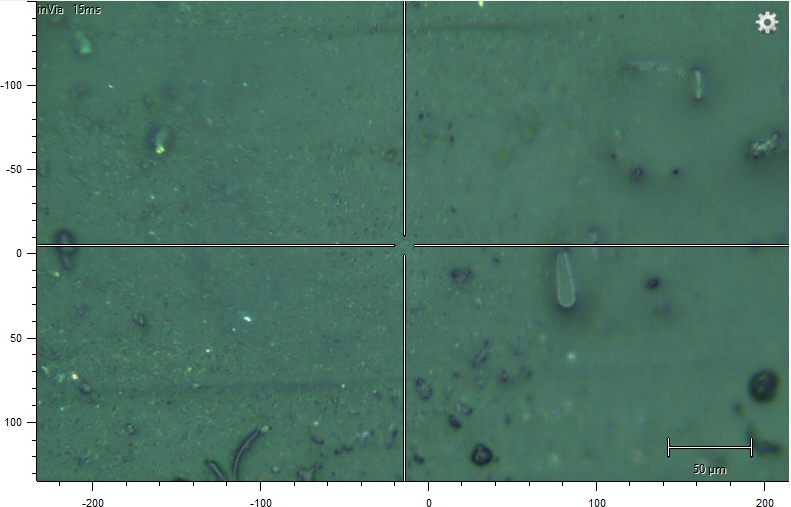
\includegraphics[width=0.4\linewidth]{Figures/Raman_still_9CBSR_50x_loc5.jpg}
%	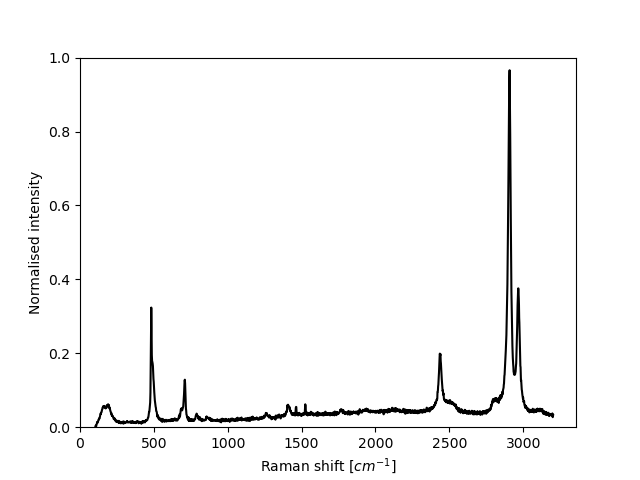
\includegraphics[width=0.4\linewidth]{Figures/Raman_0CBSR_10s_LP1_AC1_50x_loc1.png}
%	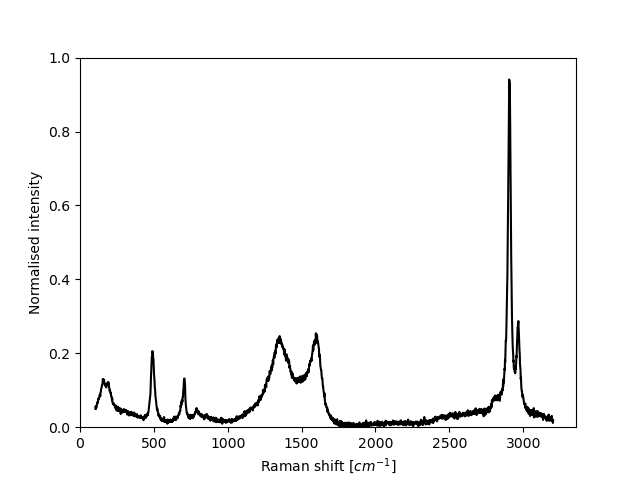
\includegraphics[width=0.4\linewidth]{Figures/Raman_8CBSR_10s_LP5_AC1_20x_loc1.png}
%	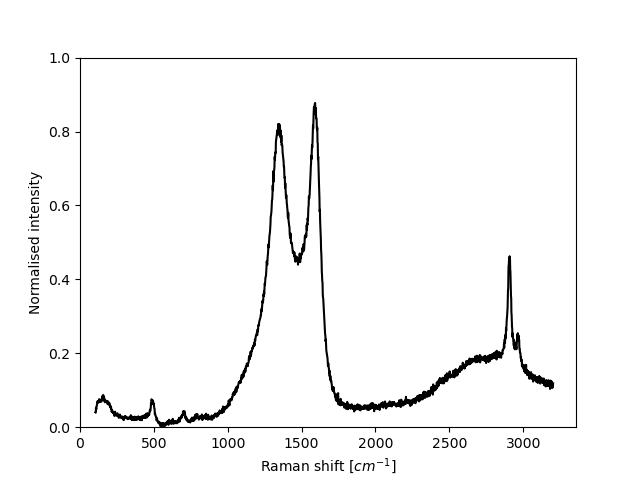
\includegraphics[width=0.4\linewidth]{Figures/Raman_cut8CBSR_10s_LP5_AC1_20x_loc1.png}
	\caption{(A): Typical screenshot from the focused Raman microscope. Normalised Raman spectrum of (B) the plain SR. (C) the top surface of CBSR specimen. (D) the cross-sectional surface of CBSR specimen.}
	\label{fig:Raman_CB_SR}
\end{figure}
These plots in Figures \ref{subfig:raman_0CB} - \ref{subfig:raman_8CB_cut} show that surface electrodes will have a smaller chance of obtaining a reliable connection to the conductive network to the internal the CBSR composite, due to the low CB particle content measured at the surfaces on the specimens.

% To do: CB dispersion imaging - show Raman mapping and SAXS results. SAXS analysis may take time, and potential inclonclusive results.

\subsection{Stress-Strain-Resistance Measurement}
A custom test measurement device was made for measuring the desired characteristics of the CBSR material, so that parameters driving the data collection such as the current source and strain profile could be easily customised to suit the experiment. The strain, stress, and resistivity of the specimen were measured in in parallel. The setup included the use of a 500 g TAL221 loadcell (HT Sensor Technology Co. Limited., Xi'an, China) in combination with a linear actuator stage driven by a NEMA23 stepper motor and a 2634B Keithley source measurement unit (SMU) (Tektronix, Beaverton, USA). The loadcell was found to have a resolution of $\pm$ 30 mN and the linear actuator stage used a G201x micro-stepper controller (Geckodrive, Santa Ana, USA) allowing for 40 $\mu$m steps.
\begin{figure}[H]
	\centering
	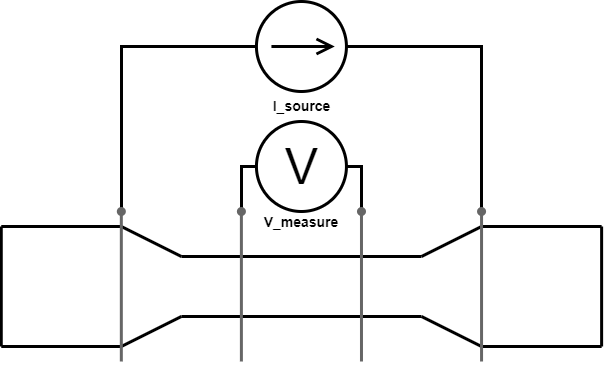
\includegraphics[width=0.5\linewidth]{Figures/4wire_specimen.png}
	\caption{The composite dog-bone test specimen pierced by 4 metal pin electrodes. The outer and inner electrodes connected to an SMU current source and voltmeter respectively}
	\label{fig:four_wire_dogbone}
\end{figure}
%Two configurations of resistance measurement were tested, a two-wire and a four-wire method. The two-wire measurement method used two copper plate electrodes which also clamped the test specimen at each end. It was observed that compressive strain applied to CBSR composite alters the resistivity of the specimen in a similar fashion to tensile stress. Only a compressive strain was applied to the material by the clamps such that the material would not slip during tensile testing and not deform giving erroneous resistance results.
%The two-wire method used a controlled current source in parallel with a voltmeter attached to the same two electrodes to measure a resistance. 
The four-wire method uses four pin electrodes as seen in Figure \ref{fig:four_wire_dogbone}. The four-wire method applies a constant current source through the outer electrodes and uses a voltmeter on the inner two electrode to determine the resistance of the specimen. The four-wire electrode configuration exhibited a larger signal-to-noise-ratio (SNR) compared to the two-wire alternative for resistance measurements. Four-wire pin electrodes were selected because they resulted in minimal specimen deformation, exhibited a high measurement SNR, no slip, and the electrode can pierce through the specimen which ensured a constant electrode impedance. The inner pin electrodes were symmetric about the centre and placed 20 mm apart with the outer pin electrodes being 40 mm apart as shown in Figure \ref{fig:electromech-setup}.
\begin{figure}[H]
	\centering
	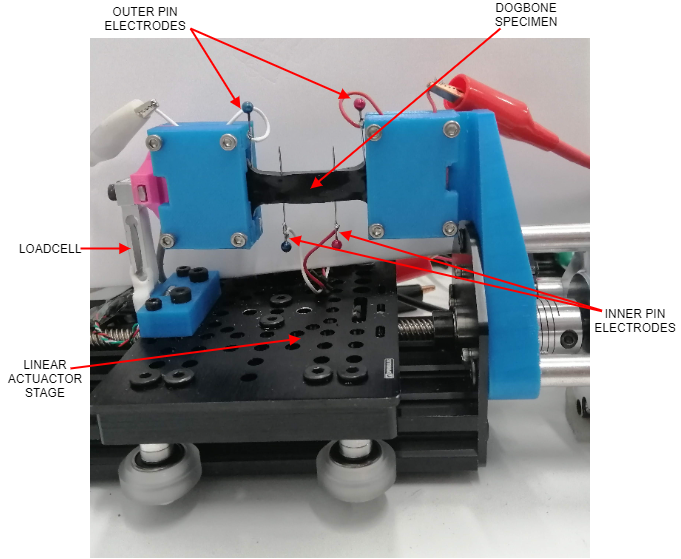
\includegraphics[width=0.7\linewidth]{Figures/ELECTROMECH-SETUP.png}
	\caption{Photo of test measurement setup}
	\label{fig:electromech-setup}
\end{figure}
The dogbone specimen was held in place using clamps with an a 3D pyramidal array surface. 
The specimen clamp strain was calculated using the specimen Poisson's ratio and the maximum expected tensile experiment strain; to ensure the specimen would not slip, and ensure minimal deformation to the specimen.
  
The measurements were completed using controlled sinusoidal, saw-tooth, and pulse trains of strain to ensure repeatability of the models were consistent across varying experimental parameters. If this material is used as a sensor the model fitted to the stress relaxation must hold over many consecutive tensile strain events. As these materials are intended as large strain sensors, the main strains tested in this work were ranged between 0 and 30\%, with a strain-rates ranging from 0 to 6.67 $\% \cdot s^{-1}$.

All data was captured through serial interfaces and logged on a PC with a python-based program. An open source G-code platform GRBL was used to control the motion of the linear actuator. The PyVISA library was used to obtain all of the measurement data and to send commands to measurement devices. A calibration procedure ensured that the stress and strain of the specimen was always zero'd before each experiment. The functional architecture of the system is shown in Figure \ref{fig:electromech-architecture}.
\begin{figure}[H]
	\centering
	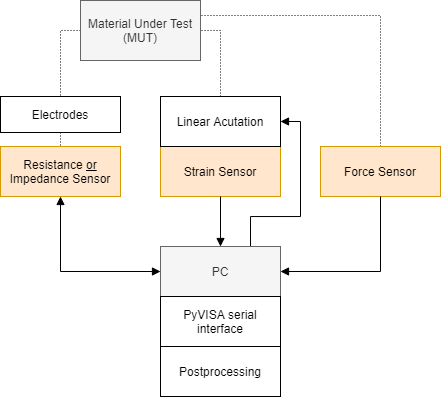
\includegraphics[width=0.65\linewidth]{Figures/Electromech_tester.png}
	\caption{System architecture for the electromechanical tensile test rig showing data/physical connections}
	\label{fig:electromech-architecture}
\end{figure}


\section{Results and Analysis}
% TODO: add some bloatage here explaining section!!
The CBSR composite material has shown complex nonlinear behaviour in previous literature as discussed in Section \ref{sec:ch3-intro}, hence a piece-wise approach to modelling the CBSR composite has been taken to describe the electromechanical dynamic behaviours of the material. To understand the transient behaviour of CPECs several dynamic repeatable electromechanical characteristics of CBSR have been classified and mathematical representations fitted. This section aims to provide repeatable mathematical relationships for several dynamic phenomena working towards creating an overarching model which combines each of the phenomena.
% See CBSR behaviours document and flesh out with data!!


\subsection{Stress-Strain and Viscoelasticity}
All of the specimens fabricated indicated a degree of viscoelasticity shown by the hysteresis seen when loading and unloading the material with 30\% tensile strain in Figure \ref{fig:loading-and-unloading-specimens}. The 0, 7.5, and 10 w.t.\% CB specimens have average elastic moduli, as measured in the loading phase, of 205.2 kPa, 321.4 kPa, and 342.1 kPa, respectively.
\begin{figure}[H]
	\centering
	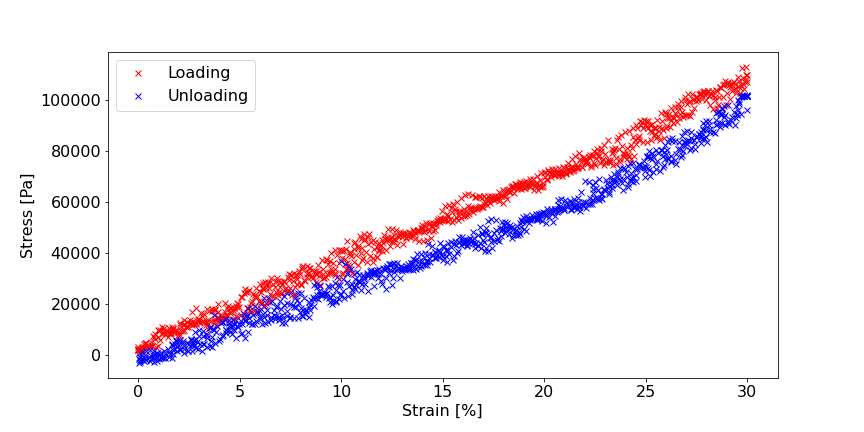
\includegraphics[width=0.69\linewidth]{Figures/load_unload_1_10_E4pin_20mm_v9_0.3Strain.png}
	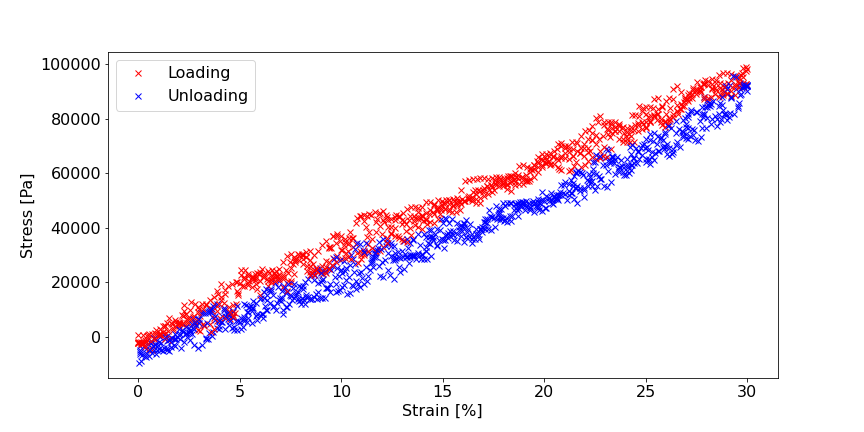
\includegraphics[width=0.69\linewidth]{Figures/load_unload_2_7-5_E4pin_20mm_v10_0.3Strain.png}
	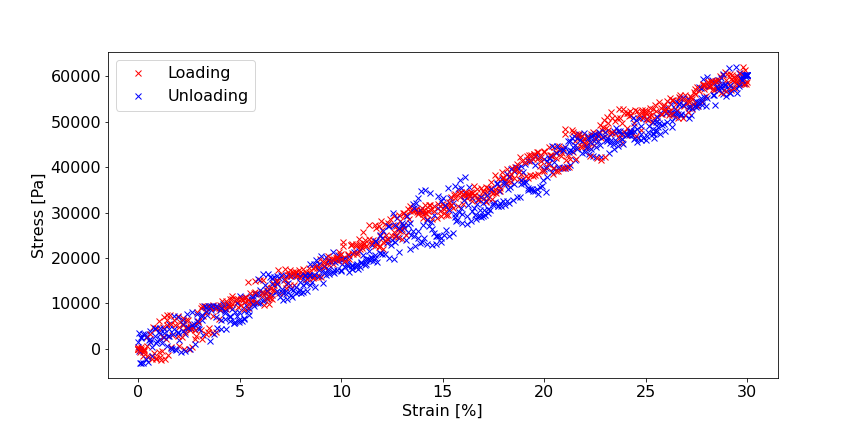
\includegraphics[width=0.69\linewidth]{Figures/load_unload_1_CB0_v1_0.3Strain.png}
	\caption{The loading and unloading of 30\% strain on a composite test specimens with CB weight percentages from top to bottom of 10\%, 7.5\%, and 0\% with data collected over five loading and unloading cycles}
	\label{fig:loading-and-unloading-specimens}
\end{figure}


\subsection{Quasi-Static Tensile Resistance-Strain}
\label{subsec:Quasi-Static Tensile Resistance-Strain}
To understand how the material could be used for a low-frequency response application the underlying steady-state relationship between resistance and strain was found by producing a quasi-static linear resistance-strain formula for strains between 0 to 30\% strain. Data was gathered using steady-state measurements from four separate tensile strain pulses performed on the same CBSR specimen as shown in Figure \ref{fig:quasi_static_tensile}.
\begin{figure}[H]
	\centering
	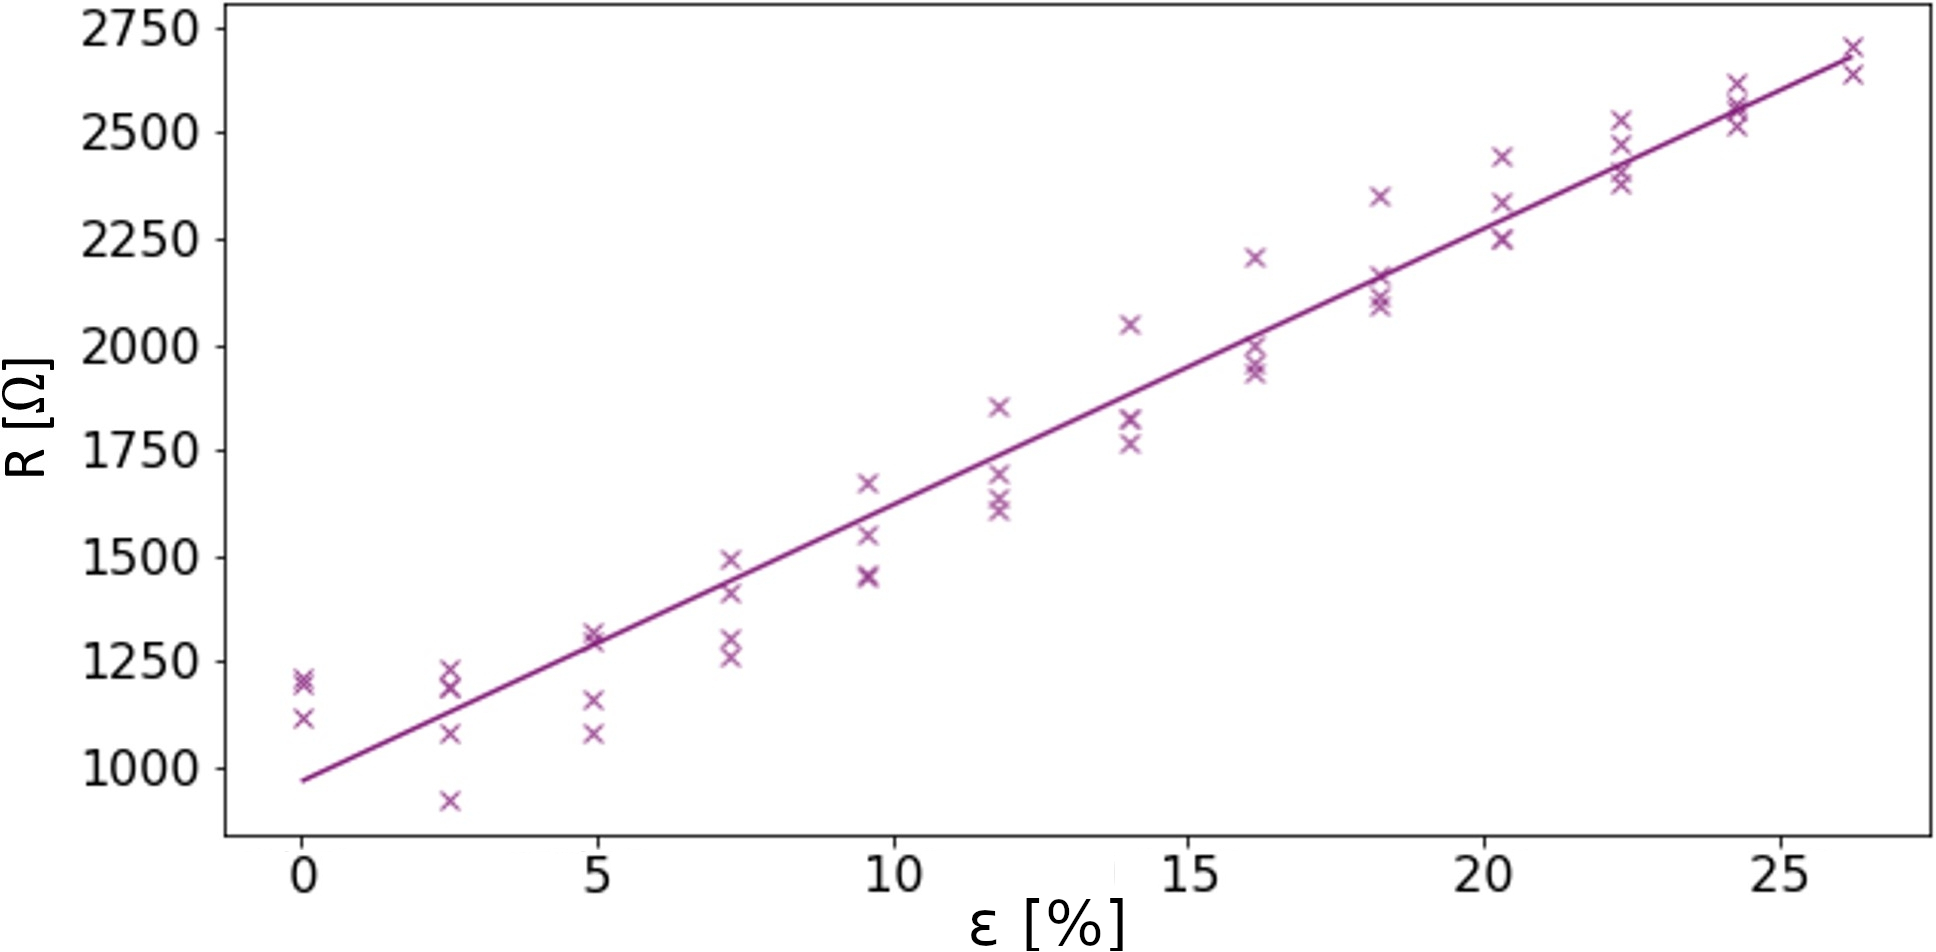
\includegraphics[width=0.8\linewidth]{Figures/2_7-5_4Epin_20mm_v2_Quasi_static_fit.jpg}
	\caption{Linear quasi-static resistance-strain fit for 7.5 w.t.\% CBSR specimen}
	\label{fig:quasi_static_tensile}
\end{figure}
The fitted parameters for the linear quasi-static model are given in Equation \ref{eqn:quasi-R-strain_7-5}.
\begin{equation}
	R = 6530 \cdot \varepsilon + 970
	\label{eqn:quasi-R-strain_7-5}
\end{equation}


\subsection{Dynamic Resistance-Strain-Rate Response}
When using this material as a tensile strain sensor many applications will require a strain-rate superseding the capabilities of the quasi-static model given in Section \ref{subsec:Quasi-Static Tensile Resistance-Strain} due to the resistive relaxation in the material characterised in Section \ref{subsec:resistive relaxation Fitting}. The dynamic characteristics of the CBSR material is investigated to find a relationship between the strain-rate and resistance. Several saw-tooth strain signal experiments were completed using four different strain-rates of 1.67, 3.33, 5, and 6.67 \%$\cdot$s$^{-1}$. To avoid measuring a time-dependent relationship in stead of the desired strain-rate dependent relationship, each set of different strain-rates were repeated as shown in Figure \ref{fig:saw-tooth-diff-v}.
\begin{figure}[H]
	\centering
	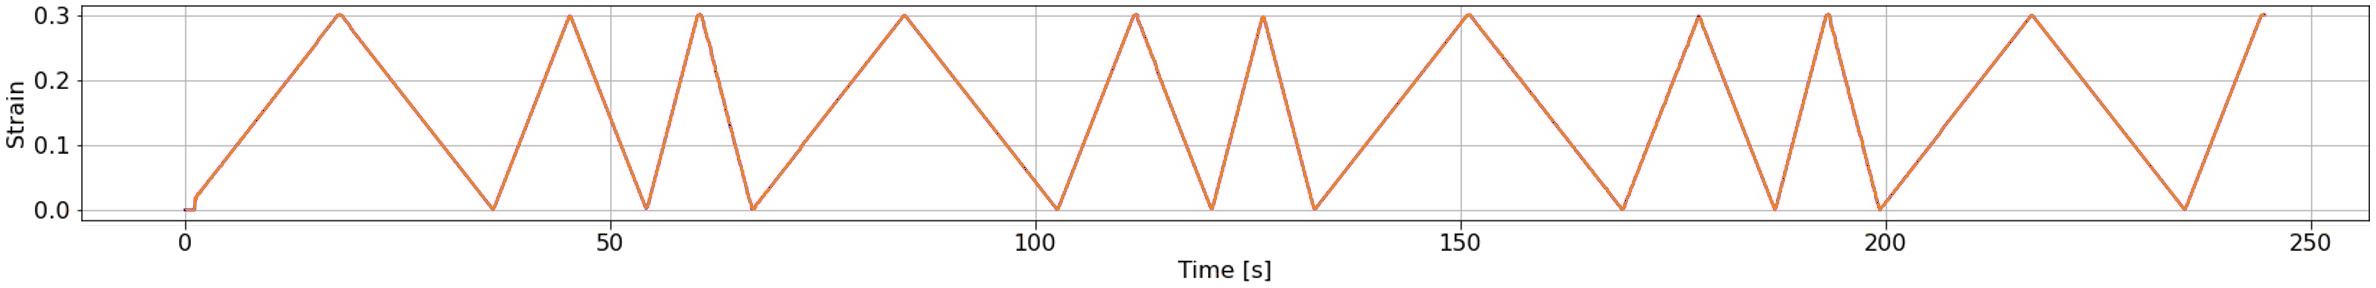
\includegraphics[width=\linewidth]{Figures/saw_tooth_diff_speeds_strain_only.jpg}
	\caption{Strain input waveform for investigating strain-rate dependent resistance}
	\label{fig:saw-tooth-diff-v}
\end{figure}
The resulting resistance response exhibits a shoulder peak phenomena where a second peak is developed when suddenly decreasing the strain-rate. The resistance response is shown in Figure \ref{fig:saw-tooth-res-response}.
\begin{figure}[H]
	\centering
	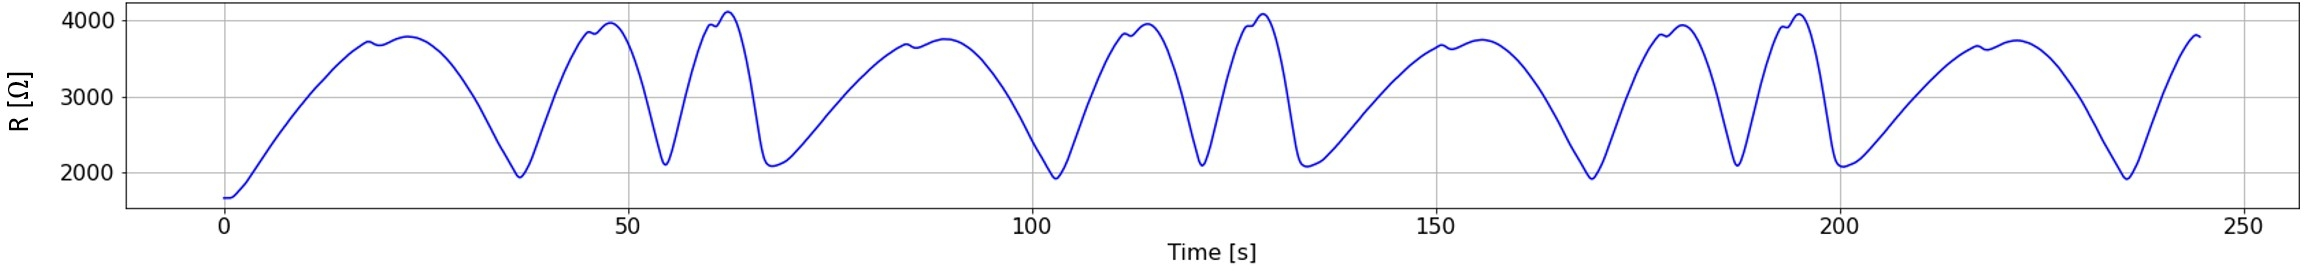
\includegraphics[width=\linewidth]{Figures/saw_tooth_diff_speeds_res_only.jpg}
	\caption{Resistance response from saw-tooth strain input Figure \ref{fig:saw-tooth-diff-v}.}
	\label{fig:saw-tooth-res-response}
\end{figure}
Hysteresis loops were used in Figure \ref{fig:saw-tooth-hysteresis-loops} to show resistance offset as a function of the strain-speed and simultaneously displaying the resistance hysteresis loops of different strain speeds. 
\begin{figure}[H]
	\centering
	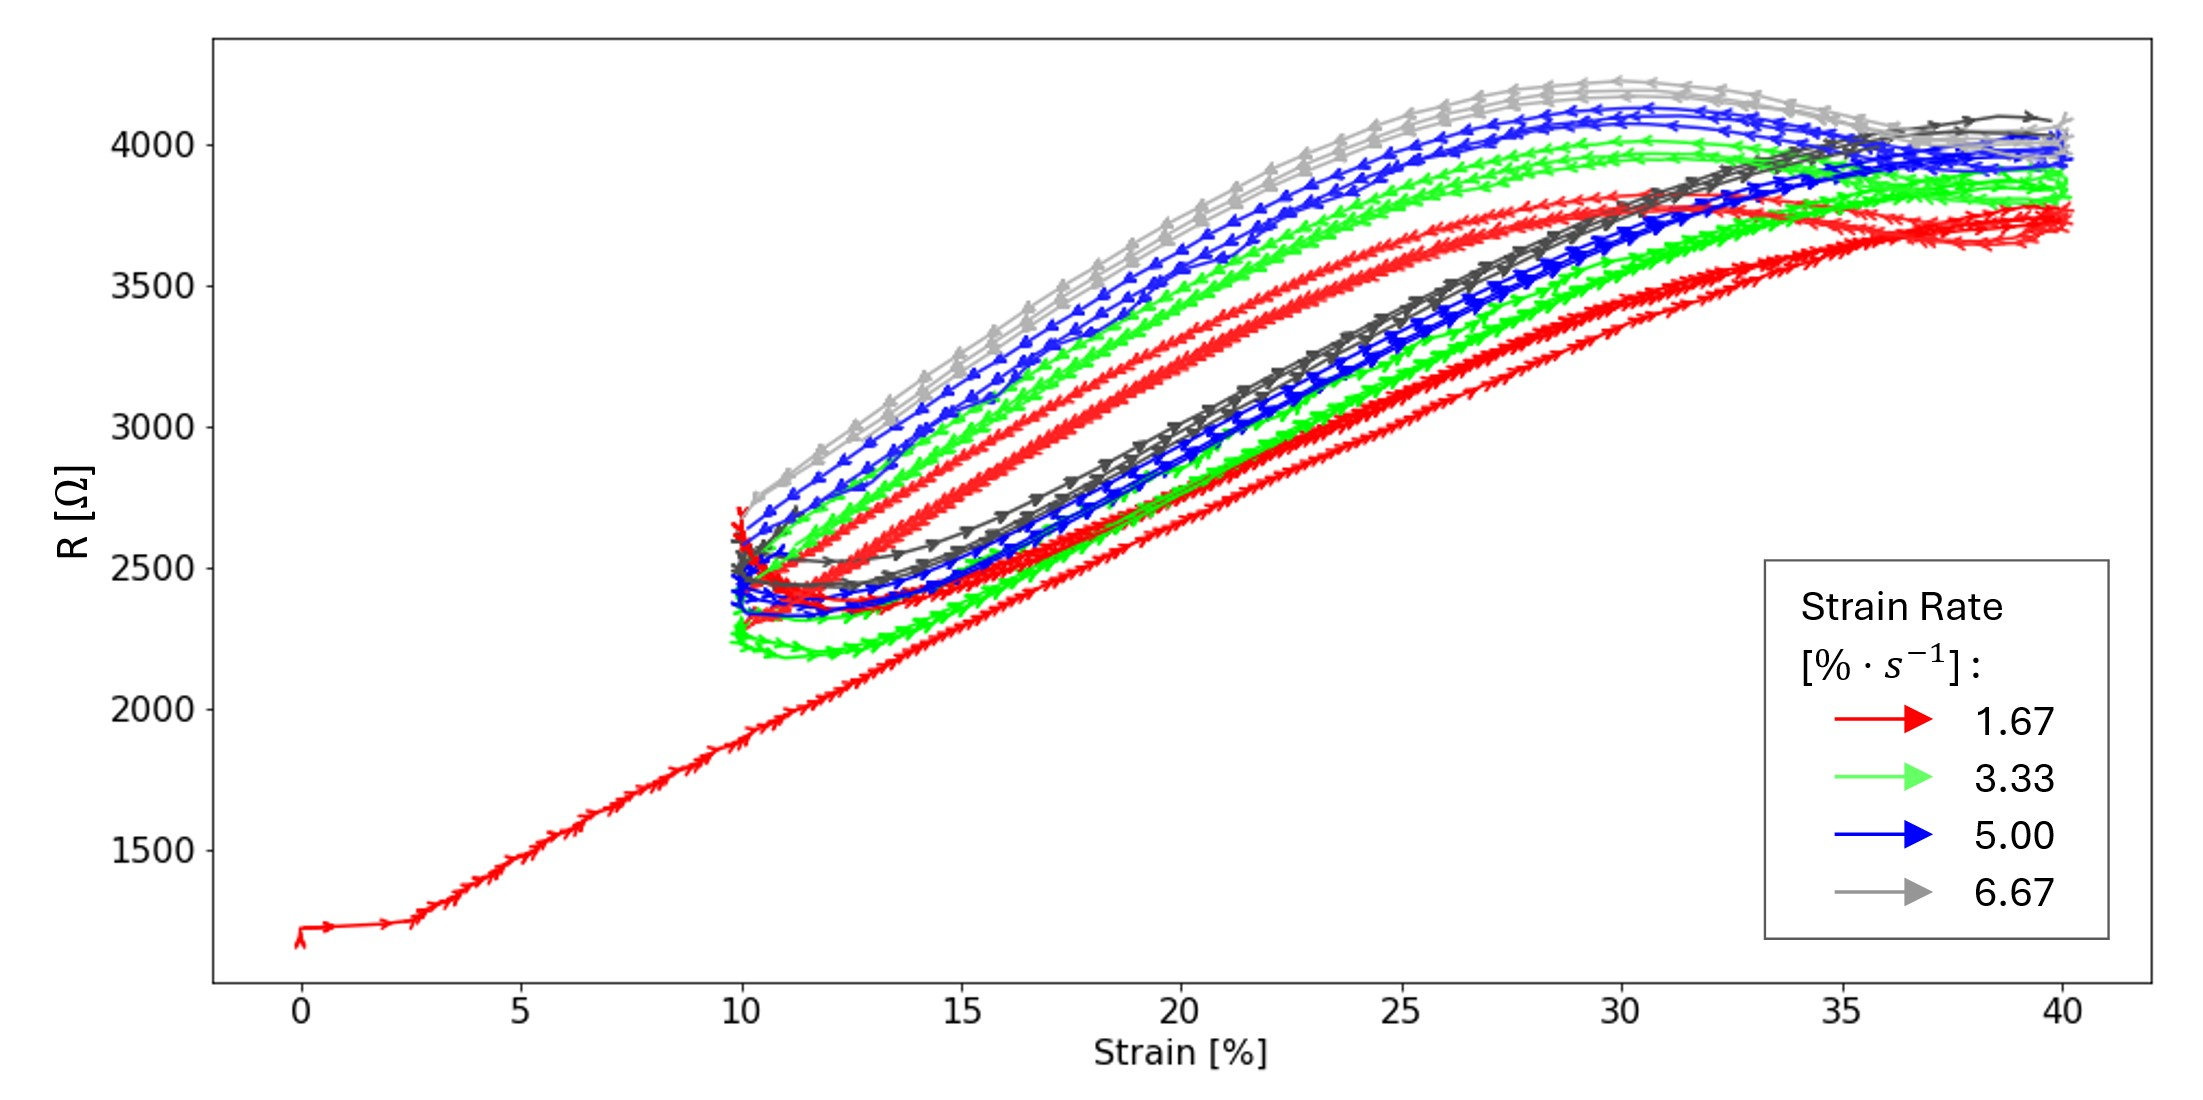
\includegraphics[width=\linewidth]{Figures/hysteresis_strain_varSpeeds_ledge_corrected.jpg}
	\caption{Resistance vs strain hysteresis loops from from a saw-tooth strain input.}
	\label{fig:saw-tooth-hysteresis-loops}
\end{figure}
The material was pre-strained to mitigate non-linear effects that may arise near 0\% strain. Using the 1.67 \%$\cdot$s$^{-1}$ strain-rate as a reference the average resistance offset of the other three strain-rates tested were calculated as shown in Table \ref{tab:rel-dR-strain-rate}.
\begin{table}[H]
	\centering
	\caption{Strain-rate dynamic resistance offset comparison. Using S1 as the reference resistance loop.}
	\label{tab:rel-dR-strain-rate}
	\begin{tabular}{c|cccc}
		Strain-rate \# & S1 & S2 & S3 & S4 \\
		\hline
		$\dot\varepsilon$ $[\%\cdot s^{-1}]$ & 1.67 & 3.33 & 5.00 & 6.67 \\
		\hline
		$\Delta R_{S1}$ [\%] & 0 & +5.0 & +8.3 & +10.7 \\
		% \hline
	\end{tabular}
\end{table}


\subsection{Falling Edge Strain-Rate-Resistance}
A narrow peak in the measured resistance has been observed in the collected data when during a falling edge. This peak is not present in the stress plot shown in Figure \ref{fig:stress_strain_res_pulse}, hence is a proposed characteristic of electrical behaviour only as a function of strain as the change is resistance is assumed to be primarily due to conductive particle motion.
\begin{figure}[H]
	\centering
	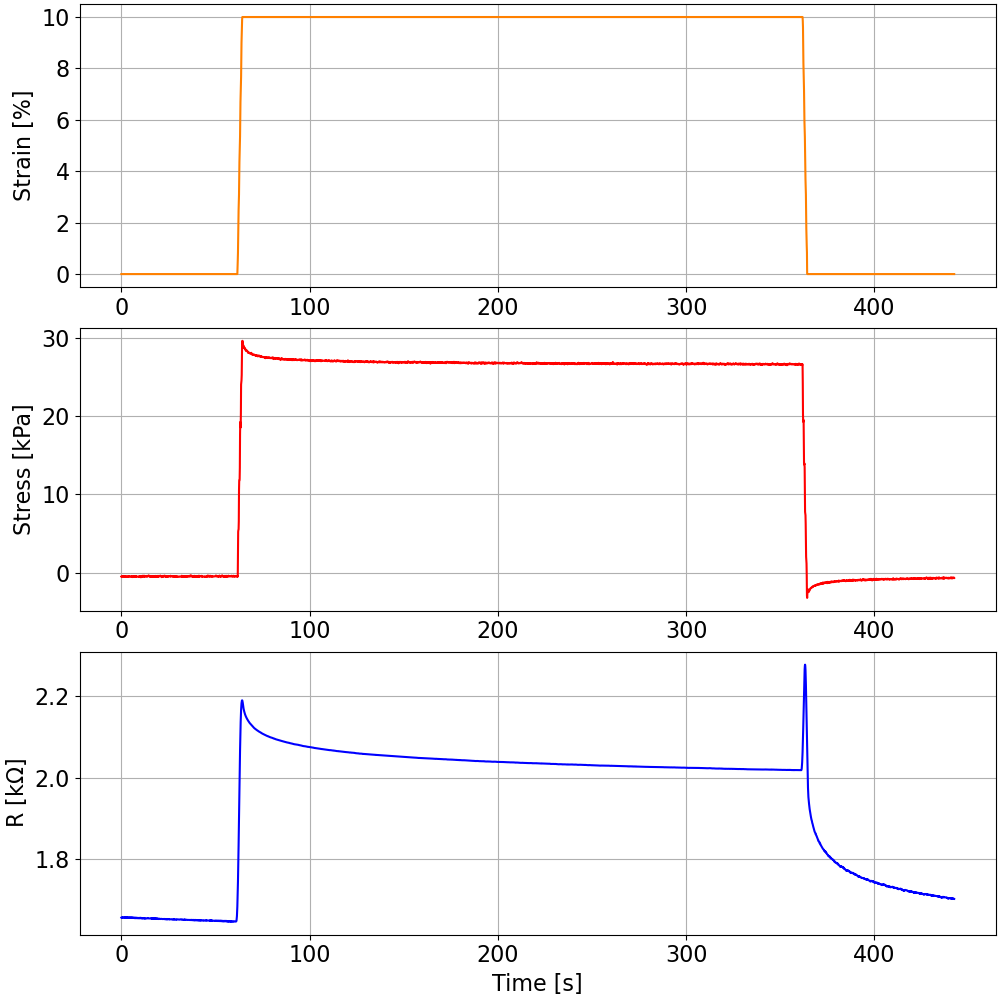
\includegraphics[width=0.6\linewidth]{Figures/2_7-5_E4pin_20mm_v6_stress_strain_res_pulse.png}
	\hspace{1cm}
	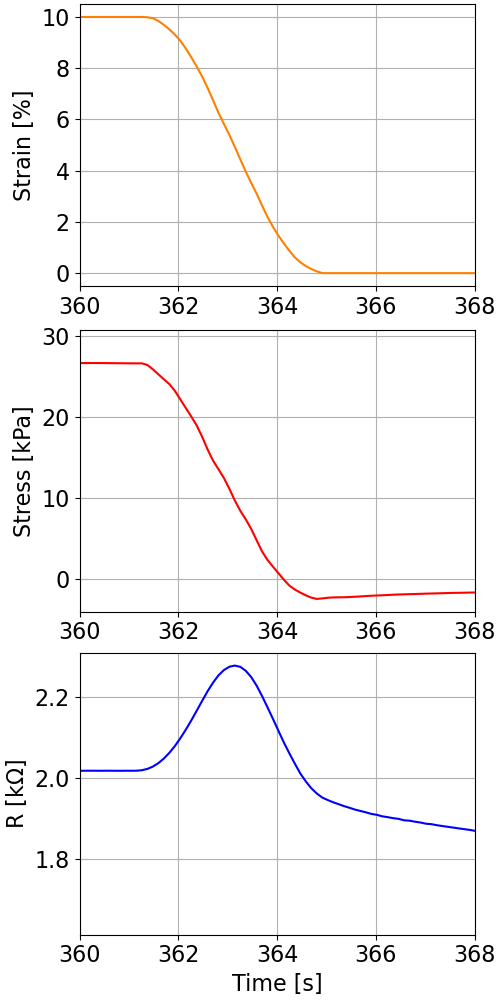
\includegraphics[width=0.3\linewidth]{Figures/2_7-5_E4pin_20mm_v6_stress_strain_res_pulse_f-edge.png}
	\caption{Left: Singluar tensile strain pulse with resulting stress and resistance reponse. Right: Zoomed to higlight falling edge shoulder phenomena.}
	\label{fig:stress_strain_res_pulse}
\end{figure}
A parameter fit study has been completed to determine the resistance peak amplitude can be determined with a range of  strain-rates. We can see a repeated phenomena in Figure \ref{fig:poly2_r_strain} whereby the derivative of the resistance signal seems to be equal to the strain curve. The resistance peak curve, $R_p$, can be modelled with a second order polynomial. When differentiated, this peak gives a linear function in a similar form of the linear strain curve seen in Figure \ref{fig:poly2_r_strain}. Hence we form Equation \ref{eqn:dR_dt_strain} which relates resistance to strain as a function of time.
\begin{equation} 
	%TODO: Double check this equation makes sense.
	\frac{dR_p}{dt} = J(\varepsilon) \cdot t + c
	\label{eqn:dR_dt_strain}
\end{equation}
where $J$ is a function of strain, $\varepsilon(t)$, and c is an offset bias determined by the initial strain condition.
\begin{figure}[H]
	\centering
	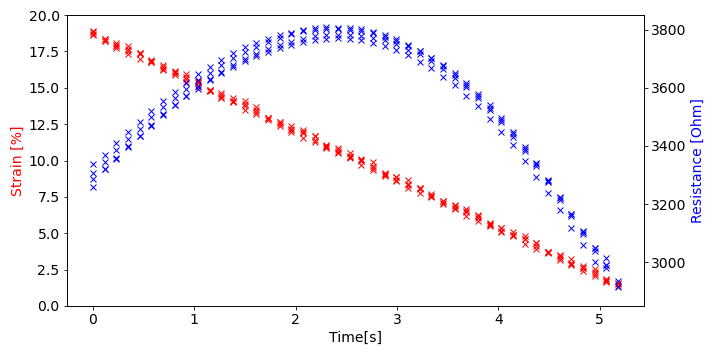
\includegraphics[width=0.8\linewidth]{Figures/strain_velocity_res_80mms_2_7-5_E4pin_20mm_v11_0.2Strain_velocityprof.png}
	\caption{Strain-rate resistance relationship showing the specimen returning to a 0\% tensile strain state from 10\% at a strain-rate of 3.33\%$\cdot s^{-1}$ from four tests for a 7.5\% CBSR specimen}
	\label{fig:poly2_r_strain}
\end{figure}
To show the strain-rate resistance relationship, more strain pulse train tests of 20\% strain were completed. Using 20\% strain allowed observation of sufficient data points to observe a trend. The pulses had four repetitions with a range of strain-rates, $\dot{\varepsilon}(t)$, of 1.67, 3.33, 5.00, and 6.67 \%${\cdot s^{-1}}$. Using a 7.5 w.t.\% CBSR specimen we obtain a relationship that agrees with the strain resistance component equation \ref{eqn:dR_dt_strain}. As $\dot{\varepsilon}(t)$ increases through strain-rates in parallel with the magnitude of the resistance peak relative to the previous steady state of value resistance. Two formulae are fitting to the linear strain and resistance peak features given by Equations \ref{eqn:strain-t-lin-fit} and \ref{eqn:res-t-ploy2-fit} respectively.
\begin{equation}
	\varepsilon = A \cdot t + B
	\label{eqn:strain-t-lin-fit}
\end{equation}
\begin{equation}
	R_{peak} = C \cdot (t - D)^2 + E
	\label{eqn:res-t-ploy2-fit}
\end{equation}
The resulting plots fitting of the averaged data points for the strain and resistance peak curves are given in Figure \ref{fig:poly2_strain_relation}.
\begin{figure}[H]
	\centering
	\begin{minipage}[t]{.49\textwidth}
		\centering
		\subfloat[][$\dot\varepsilon = 1.67 \% s^{-1}$]{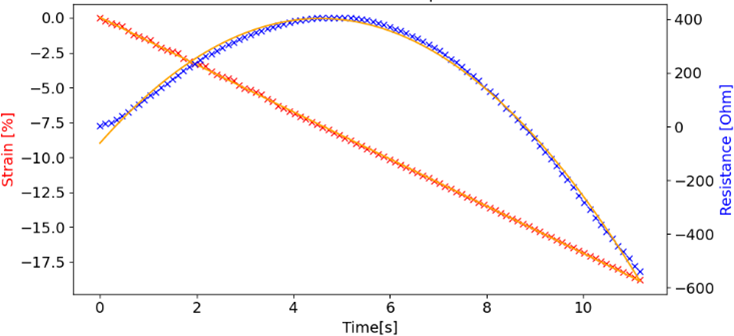
\includegraphics[width=\textwidth]{Figures/fitted_strain-r-strain-rate_1.67.png}\label{subfig:strain-rate-1.67}}
		\vfill
		\subfloat[][$\dot\varepsilon = 3.33 \% s^{-1}$]{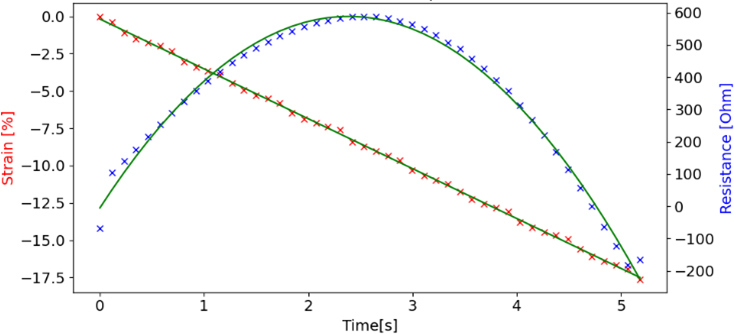
\includegraphics[width=\textwidth]{Figures/fitted_strain-r-strain-rate_3.33.png}\label{subfig:strain-rate-3.33}
		}
	\end{minipage}
	\begin{minipage}[t]{.49\textwidth}
		\centering
		\subfloat[][$\dot\varepsilon = 5.00 \% s^{-1}$]{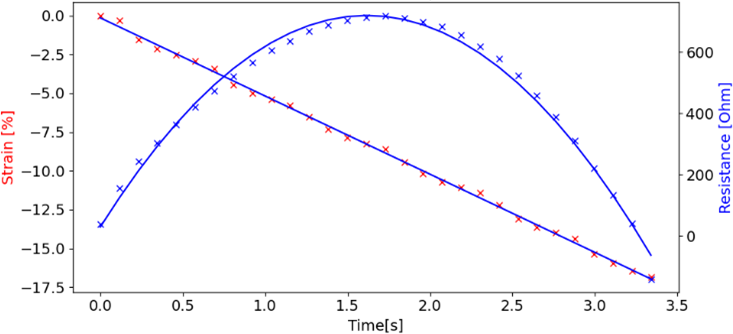
\includegraphics[width=\textwidth]{Figures/fitted_strain-r-strain-rate_5.00.png}\label{subfig:strain-rate-5.00}}
		\vfill
		\subfloat[][$\dot\varepsilon = 6.67 \% s^{-1}$]{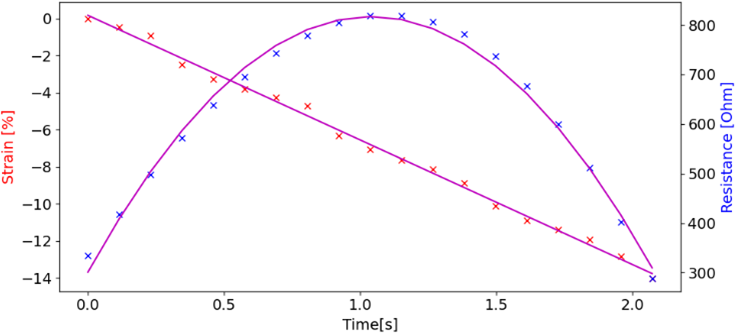
\includegraphics[width=\textwidth]{Figures/fitted_strain-r-strain-rate_6.67.png}\label{subfig:strain-rate-6.67}}
	\end{minipage}
	\caption{Fitting curves to a range of different tensile falling edge strain strain-rates.}
	\label{fig:poly2_strain_relation}
\end{figure}
\begin{table}[H]
	\centering
	\caption{The fitted parameters for relationship between the specimen tensile strain-rate the resulting resistance peak for a strain signal falling edge.}
	\label{tab:}
	\begin{tabular}{lllll}
		\hline
		\textbf{Strain rate [\%/s]} & \textcolor{orange}{\textbf{--- 1.67}} & \textcolor{ForestGreen}{\textbf{--- 3.33}} & \textcolor{blue}{\textbf{--- 5.00}} & \textcolor{Rhodamine}{\textbf{--- 6.67}} \\ \hline
		\textbf{A} ($\mathbf{\times 10^3}$) & -16.83 ± 0.09 & -33.40 ± 0.02 & -50.34 ± 0.36 & -66.82 ± 0.37 \\ \hline
		\textbf{B} ($\mathbf{\times 10^3}$) & -0.45 ± 0.93 & -0.69 ± 1.20 & -1.77 ± 1.72 & -0.13 ± 2.15 \\ \hline
		\textbf{C} & -22.10 ± 0.55 & -103.19 ± 2.30 & -250.40 ± 9.95 & -478.81 ± 32.87 \\ \hline
		\textbf{D} & 4.58 ± 0.02 & 2.37 ± 0.02 & 1.60 ± 0.06 & 1.12 ± 0.05 \\ \hline
		\textbf{E} & 403.27 ± 13.52 & 586.87 ± 23.46 & 711.96 ± 7.19 & 809.21 ± 26.46 \\ \hline
	\end{tabular}
\end{table}

%To prove that there does exist a mathematical relationship between the two signals the relationship first each signal is given a generalised formula. The resistance signal is parabolic Equation \ref{eqn:gen_parabolic}. 
%\begin{equation}
%	R_p = A \cdot (t-H)^2 + K
%	% A : concavity
%	% H : horizontal shift
%	% K : vertical shift
%	\label{eqn:gen_parabolic}
%\end{equation}
%Where strain-rate changes the vertical shift, K, time shift, H, and concavity, A, of the parabola. 

\subsection{Resistive Relaxation Fitting}
\label{subsec:resistive relaxation Fitting}
The initial model chosen to fit the stress and resistive relaxation data was the generalised Maxwell body model shown in Figure \ref{eqn:Maxwell_general} with n = 3 cascading elements using Equation \ref{eqn:Maxwell_general_3elementS} to fit the model. Fitting the data using Levenberg–Marquardt non-linear least square algorithm over 30 data sets showed an instability with the algorithm using this model. When feeding the previously fitted stress relaxation model parameters as initial conditions for the fitting of the next stress relaxation data set, the values of the parameters diverged exhibiting signs of overfitting. This divergence of the model parameters gave a large standard deviation showing the model was changing significantly each iteration of fitting. Hence a more simple model using Equation \ref{eqn:Maxwell_general} with n = 2 was used to fit the stress relaxation data to Equation \ref{eqn:Maxwell_general_2elementS} with lower standard deviation of the model constants. Conversely when the resistive relaxation model analogous to stress relaxation model, shown in Equation \ref{eqn:Maxwell_general_3elementR}, was fitted to the resistive relaxation data there was a stable fit with an improved goodness of fit.

The decay time constants of the two models are different with the resistance having an longer overall decay which can clearly be seen in Figure \ref{fig:diff_tau_res_stress}. Below in stress relaxation models $G_{1,2}(t)$, shown in Equation \ref{eqn:Maxwell_general_3elementS} and \ref{eqn:Maxwell_general_2elementS}, the constants $a_{0-3}$ and $\tau_{S1-S3}$ represent the components of magnitude and time decay of the stress relaxation, respectively.
\begin{equation}
	G_1(t) = a_0 + a_1e^{-t/\tau_{S1}} + a_2 \cdot e^{-t/\tau_{S2}} + a_3 \cdot e^{-t/\tau_{S3}}
	\label{eqn:Maxwell_general_3elementS} 
\end{equation}
\begin{equation}
	G_2(t) = a_0 + a_1 \cdot e^{-t/\tau_{S1}} + a_2 \cdot e^{-t/\tau_{S2}}
	\label{eqn:Maxwell_general_2elementS} 
\end{equation}
Analogously for the resistive relaxation function $H(t)$, the constants $b_{0-3}$ and $\tau_{R1-R3}$ represent the components of magnitude and time decay of the resistive relaxation, respectively. 
\begin{equation}
	H(t) = b_0 + b_1 \cdot e^{-t/\tau_{R1}} + b_2 \cdot e^{-t/\tau_{R2}} + b_3 \cdot e^{t/\tau_{R3}}
	\label{eqn:Maxwell_general_3elementR} 
\end{equation}
\begin{figure}[H]
	\centering
	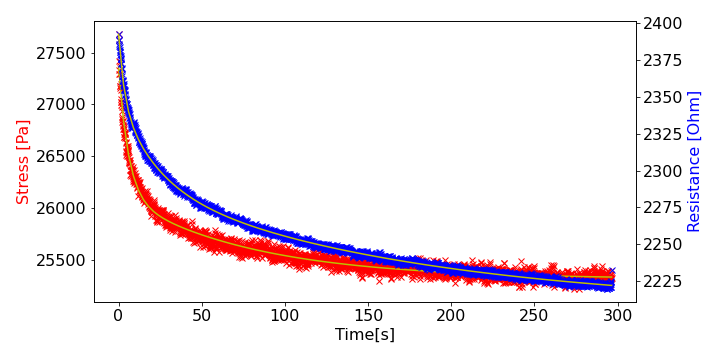
\includegraphics[width=0.9\linewidth]{Figures/diff_time_const_Res_Stress_2_7-5_Epin_20mm_v3_pulse_6.png}
	\caption{Comparing the relaxation decay time constants of stress and resistance for a 7.5 w.t.\% CBSR composite after a 10\% strain step input and fitting generalised maxwell body models to each.}
	\label{fig:diff_tau_res_stress}
\end{figure}
The mean magnitude and decay time constants for the resistance and stress relaxations using 30 relaxation periods to fit the models to are given in table \ref{tab:generalised_model_constants}.

% \newpage
\begin{table}[H]
	\caption{Fitted constants and their mean, $\mu$, standard deviation values for 0\%, 7.5\%, and 10\% CBSR composite specimens using Equation \ref{eqn:Maxwell_general_2elementS}.}
	\begin{center}
		\label{tab:generalised_model_constants}
		\begin{tabular}{l l}
			\textbf{Stress Model Parameters} & \\ 
			\hline
			0 \% CB Specimen & \\ 
			\hline
			Parameter & $\mu$ \\
			\hline
			$a_0$ & 20344 $\pm$ 42 \\
			$a_1$ & 387 $\pm$ 60 \\
			$a_2$ & 527 $\pm$ 58 \\
			$\tau_{S1}$ & 72.1 $\pm$ 23.5 \\
			$\tau_{S2}$ & 5.8 $\pm$ 1.5 \\
			\hline
			7.5 w.t.\% CB Specimen & \\ 
			\hline
			Parameter & $\mu$ \\
			\hline
			$a_0$ & 25363 $\pm$ 33 \\
			$a_1$ & 802 $\pm$ 43 \\
			$a_2$ & 1242 $\pm$ 52 \\
			$\tau_{S1}$ & 71.0 $\pm$ 9.5 \\
			$\tau_{S2}$ & 5.8 $\pm$ 0.7 \\
			\hline
			10 w.t.\% CB Specimen & \\
			\hline
			Parameter & $\mu$ \\
			\hline
			$a_0$ & 32303 $\pm$ 165 \\
			$a_1$ & 1071 $\pm$ 54 \\
			$a_2$ & 1649 $\pm$ 47 \\
			$\tau_{S1}$ & 84.1 $\pm$ 10.6 \\
			$\tau_{S2}$ & 6.5 $\pm$ 0.7 \\
			\hline
		\end{tabular}
	\end{center}
\end{table}
\begin{table}[H]
	\caption{Fitted constants and their mean, $\mu$, and standard deviation values for 0\%, 7.5\%, and 10\% CBSR composite specimens using Equation \ref{eqn:Maxwell_general_3elementR}.}
	\begin{center}
		\label{tab:generalised_model_constants}
		\begin{tabular}{l l}
			\textbf{Resistance Model Parameters} & \\
			\hline
			7.5 w.t.\% CB Specimen & \\
			\hline
			Parameter & $\mu$\\
			\hline
			$b_0$ & 2154 $\pm$ 52\\
			$b_1$ & 81.1 $\pm$ 5.4\\
			$b_2$ & 56.4 $\pm$ 3.7\\
			$b_3$ & 42.2 $\pm$ 3.4\\
			$\tau_{R1}$ & 181.1 $\pm$ 33.6 \\
			$\tau_{R2}$ & 22.8 $\pm$ 3.8 \\
			$\tau_{R3}$ & 3.5 $\pm$ 0.6 \\
			\hline
			10 w.t.\% CB Specimen & \\
			\hline
			Parameter & $\mu$ \\
			\hline
			$b_0$ & 1650 $\pm$ 97\\
			$b_1$ & 55.2 $\pm$ 8.9 \\
			$b_2$ & 77.4 $\pm$ 12.2 \\
			$b_3$ & 38.4 $\pm$ 9.5 \\
			$\tau_{R1}$ & 169.6 $\pm$ 61.7 \\
			$\tau_{R2}$ & 21.9 $\pm$ 9.7 \\
			$\tau_{R3}$ & 3.0 $\pm$ 1.6 \\
			\hline
		\end{tabular}
	\end{center}
\end{table}


\subsection{Resistance-Stress Relationship}
To display the non-linear relationship between the stress and calculated resistance within the material they are plotted against each other over 30 sequential relaxation periods of 300s. The non-linear relationship between stress and resistance changes over time for each relaxation as shown in Figure \ref{fig:res_vs_stress_30pulses}, where the data for the first relaxation is displayed in green and the last relaxation in blue.
\begin{figure}[H]
	\centering
	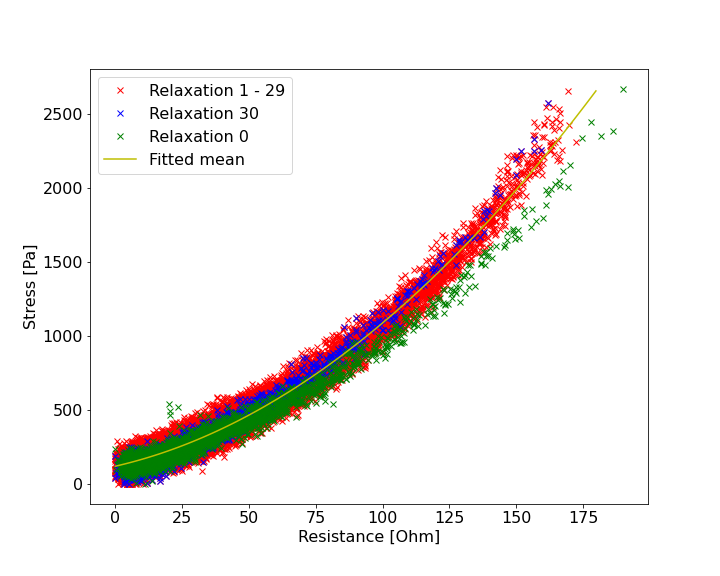
\includegraphics[width=0.7\linewidth]{Figures/relax_res_stress_non_lin_rgby_MAF8_2_7-5_Epin_20mm_v3.png}
	\caption{Comparing resistance and stress relaxation data against each other occurring during 30 pulses of a 10\% strain step input for a 7.5 w.t.\% CBSR composite}
	\label{fig:res_vs_stress_30pulses}
\end{figure}
The stress-resistive relaxation data was fitted to a generic second order polynomial of the form, 
\begin{equation}
	\sigma(R) = aR^2+bR+c
	\label{eqn:poly_res_stress}
\end{equation}
where $\sigma$ is stress, $R$ is the calculated resistance. When fit to the latter 15 cycles of a 30 cycle 10\% strain pulse train of stress relaxation data we get the constant values for $a$, $b$ and $c$.
\begin{table}[H]
	\caption{Fitted constants and their mean, $\mu$, standard deviation, $\sigma$, and coefficient of variation, $CV$, values for 7.5\%, and 10\% CBSR composite specimens using Equation \ref{eqn:poly_res_stress}}
	\begin{center}
		\label{tab:generalised_model_constants}
		\begin{tabular}{c l l l}
			7.5 w.t.\% CB Specimen \\
			\hline
			Parameter & $\mu$ \\
			\hline
			$a$ & 0.055 & 0.006 \\
			$b$ & 4.15 & 1.06 \\
			$c$ & 121.8 & 16.3 \\
			\hline
			10 w.t.\% CB Specimen \\
			\hline
			Parameter & $\mu$ \\
			\hline
			$a$ & 0.098 & 0.007 \\
			$b$ & 6.37 & 0.76 \\
			$c$ & 155.8 & 38.8 \\
			\hline
		\end{tabular}
	\end{center}
\end{table}


\section{Discussion}
This work has successfully uncovered several mathematical relationships between stress, strain, and resistance. The repeatability has also been display graphically and calculating the variance of the fitted models given. This section analyses the results given in the previous sections and highlights limitations of the experiments given.

\subsection{Fabrication}
In this work, mixing has been performed using a planetary mixer. It has been shown in other works \cite{Xu2016,Spahr2017} that other mixing methods, such as using a sonication bath and the addition of solvents, can yield more homogeneous particle dispersion. A higher degree of CB particle dispersion has also been shown to alter the viscoelastic creep properties \cite{Xu2016}, and is therefore likely to affect the time constant of resistance.

Composite imaging and experimentation showed the existence of a thin insulative film on the composite surface inhibiting the use surface electrodes to give a good electrical connection to the percolated CB network. The imaging also showed the existence of voids in the micron scale which contribute towards the material viscoelasticity. The optimisation of particle dispersion and investigation into the effects of void dispersion and sizing could give insight into maximising the material gauge factor.

When characterising the reference pure SR material, the elastic modulus was larger than the 186.2 kPa elastic modulus specified by the manufacturer, likely due to the heat assisted curing process used \cite{Johnston2014}.


\subsection{Quasi-static Tensile Resistance-Strain}
The quasi-static linear model given show promise for using the composite CBSR material for applications requiring a low frequency response sensor. This also gives a good steady-state part of a more complex model which includes the non-linear and time-dependent dynamics.


\subsection{Dynamic Resistance-Strain-Rate Response}
Increasing strain-rates were shown to increase the offsets in resistance over a range of strains as shown in Figure \ref{fig:saw-tooth-hysteresis-loops}. Showing the existence of a repeatable relationship between strain-rate and resistance, for constant strain rates. For strain acceleration different phenomena arose, such as the shoulder phenomena.


\subsection{Falling Edge Strain-Rate-Resistance}
A 'falling edge' resistance shoulder phenomena was observed and is clearly seen in Figures \ref{fig:saw-tooth-res-response} and \ref{fig:stress_strain_res_pulse}. This is a result of a change in strain rate. The amplitude of this peak was shown to increase with an increasing change in strain-rate from a steady state strain. The shoulder phenomena may existing on the rising edge of the strain adding to the resistive relaxation response however this was not easily distinguishable. In previous literature, the effects of the strain-rate and sudden change in strain-rate on apparent resistance of the CBSR material has not been modelled or shown. Another characteristic of the falling edge shoulder phenomena is the apparent positive correlation between the strain magnitude prior to the falling edge and the amplitude of the shoulder phenomena, as shown below in Appendix \ref{appendix-B}. Another characteristic of note is that the shoulder phenomena is almost not present on a falling edge that goes from a tensile (positive) strain to a small compressive (negative) strain which is also shown in Figure \ref{fig:strain-hill}.


\subsection{Resistive Relaxation Fitting}
The generalised Maxwell model has been applied to predict the stress relaxation of the CBSR composite and analogously the resistive relaxation seen for a positive strain step input. The data gathered show that the stress relaxation time constant values decrease with an increasing CB percentage, indicating that all constants in Equations \ref{eqn:Maxwell_general_3elementR} and \ref{eqn:Maxwell_general_2elementS} are also functions of CB percentage. The repeatability of this stress relaxation for strain step inputs shows promise to use of this material in controlled environments, such as factory production lines, where there are known periodic strain step inputs. An application for the resistive relaxation decay time characterisation could be for timer with a soft robotic system.

One aim of this work was to prove the hypothesis that the stress relaxation time constant is different to that of the observed resistive relaxation and able to be modelled mathematically. The apparent difference in time constants and the fitting of the data to two different equations show that the stress relaxation is not linearly related to the resistive relaxation shown clearly in Figure \ref{fig:diff_tau_res_stress}.


\subsection{Resistance-Stress Relationship}
A common hypothesis for the resistive relaxation phenomena is that it may be correlated to the resistive relaxation. This work found that the relationship between the two variables, resistance and stress, during relaxation events was non-linear and time-dependent. This non-linearity was found to have a good fit to a second order polynomial as shown in Figure \ref{fig:res_vs_stress_30pulses}. The Mullin's effect was evident in the results and a time-dependence where the concavity of the polynomial fitted increased after the first strain pulse.


\subsection{Viscoelasticity}
% see CBSR behavious doc for more hysteresis quantification
The hysteresis loop seen in the 10 w.t.\% CB sample has a larger hysteresis loop showing that there is increased viscous/damping compared with the other two specimens percentages of CB. The pure SR specimen had no discernible hysteresis from the data as shown in Figure \ref{fig:loading-and-unloading-specimens}.  The difference in hysteresis and hence viscolelastic properties, across the specimens leads to different stress relaxation properties across the three different percentages of CB composite materials in this work.


\subsection{Repeatability}
The resistive relaxation model must be predictable over many strain cycles for use within high-stretch strain sensor applications. If the resistive relaxation changes over time this needs is to be modelled. Each test sequence showed that there was a downward trend in the calculated magnitude of resistance for each pulse over time. 

The physical phenomena driving this downward trend in resistance magnitude was theorised to have two possible causes. The first cause being; the accumulation of charge within material over time generated by current source, due to the CBSR material having an RC-network-like behaviour. The second potential cause being; the gradual alignment of the CB particle network due to the electrostatic attraction of CB chains. This could be tested by increasing the current used and observing the gradient of the downward trend.

The charging theory was mitigated by using an alternating polarity measurement technique. The reversible current source was switched at 10 Hz dampened this downward trend, however the downward trend in resistance was still observed as shown in Figure \ref{fig:repeatability_pulse_trains}. An example of an experiment with the previous non-switched DC current is shown in Appendix Figures \ref{fig:strain-train-DC-meas} and \ref{fig:res-AC-DC} for comparison.
\begin{figure}[H]
	\centering
	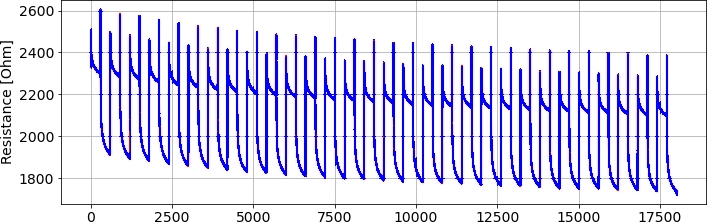
\includegraphics[width=0.6\linewidth]{Figures/30_pulse_AC_2-7-5_Epin_20mm_v3_res.jpg}
	\vspace{0.2cm}
	\vfill
	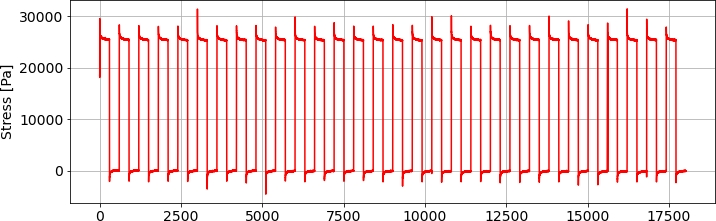
\includegraphics[width=0.6\linewidth]{Figures/30_pulse_AC_2-7-5_Epin_20mm_v3_stress.jpg}
	\vspace{0.2cm}
	\vfill
	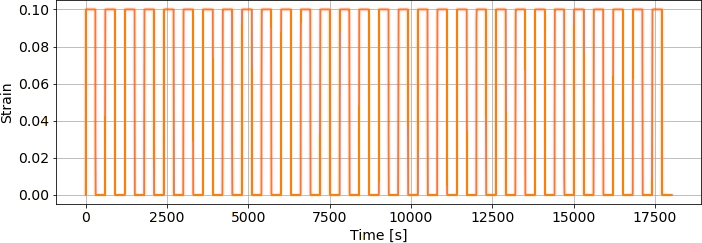
\includegraphics[width=0.59\linewidth]{Figures/30_pulse_AC_2-7-5_Epin_20mm_v3_strain.jpg}
	%	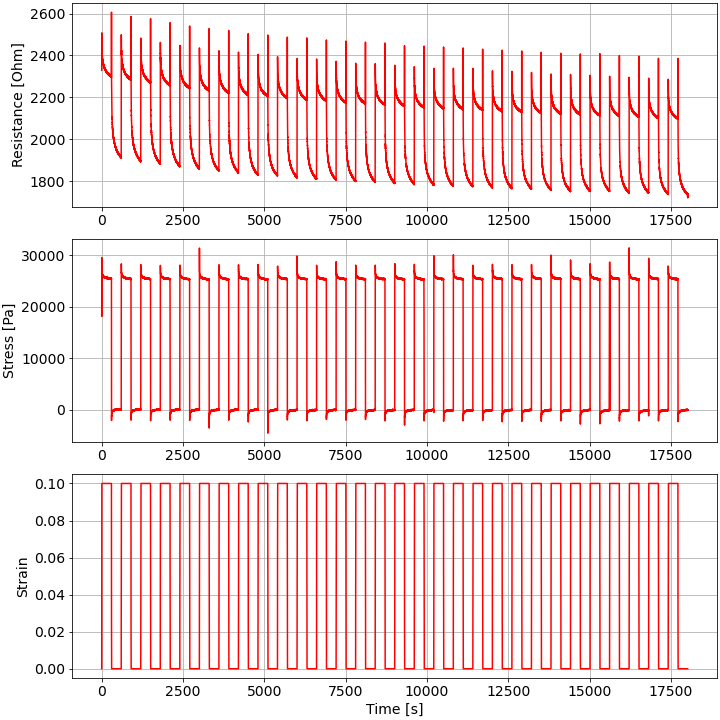
\includegraphics[width=9cm]{Figures/30_pulse_AC_2-7-5_Epin_20mm_v3.png}
	\caption{A typical test sequence of a 30 pulse strain train recording the calculated resistance and stress of a 7.5 w.t.\% CBSR composite}
	\label{fig:repeatability_pulse_trains}
\end{figure}


\subsection{Further Discussion and Future Work}
%%% place the below blurbs in the appropriate sections above.
It must be noted that for fitting the resistive relaxation, stress-resistive relaxation and the falling edge phenomena the data was translated in the xy axes for for ease of the regression algorithm fitting.

A sufficiently high current source value was required to ensure a SNR that would not hinder data analysis. There seemed to be a wetting current threshold where the SNR dropped as shown by the 20 $\mu$A resistance pulse response in Figure \ref{fig:multi_current}.
\begin{figure}[H]
	\centering
	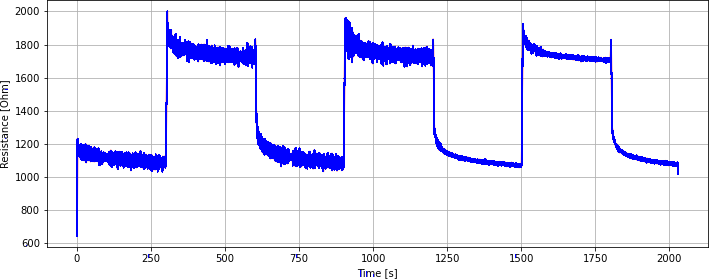
\includegraphics[width=0.7\linewidth]{Figures/test_multicurrent_2_7-5_v3_res_only.png}
	\caption{Three identical 15\% strain pulses at three different current values ,in order, 10$\mu$A, 15$\mu$A, and 20$\mu$A.}
	\label{fig:multi_current}
\end{figure}

A limitation of using this material as a strain sensor is the non-linearity of the material above a certain strain value, at which the composite's resistivity diverges towards a highly insulative value within the giga-ohms range. This non-linear behaviour of CBSR can be used as a mechanically activated switching device \cite{Henke2018}. If modelled, this non-linearity could extend the range of strains that can be measured.

The consideration of temperature and strain history \cite{Fung1993} could be used in further research to characterise a CBSR-based strain sensor for a range of application environments.

Future work includes creating a model that incorporates all of the behaviours shown in this work so that an accurate inverse model can be created to use the material as a strain sensor. To capture all of these phenomena models that can capture and recreate time-dependent phenomena such as recurrent neural networks (RNNs) could be used.

%The capacitance read across the inner pin electrodes of the material decreased with increasing strain as shown in Table \ref{tab:capacitance_v_strain}.
%%% To do: Unsure how conclusive this is... could be an incresaingly poor electrode connection impedance??
%\begin{table}[H]
%	\centering
%	\caption{Average inner electrode capacitances, $C_{in}$, measured for various strain, $\varepsilon$, values using a 7.5 w.t.\% CBSR composite, measured using an LCR meter at 1 kHz and 10 kHz \newline}
%	\label{tab:capacitance_v_strain}
%	\begin{tabular}{c|cccc}
%		% \hline
%		$\varepsilon [\%]$ & 0 & 10 & 20 & 30 \\
%		\hline
%		$C_in [pF]$ & 53 & 32 & 24 & 20 \\
%		% \hline
%	\end{tabular}
%\end{table}

\section{Conclusions}
The CBSR material used in this work provided exaggerated non-linear effects compared to literature where these non-ideal phenomena are often quashed and ignored. The relationships discussed in this work could be used to define a CBSR-based strain sensor models and show the expected behaviours in the composite material for different strain application scenarios. 

In order to improve the accuracy of dynamic strain measurements with CBSR composites a stress and analogous resistive relaxation model was formed. The generalised Maxwell model, Equation \ref{eqn:Maxwell_general_2elementS} was used to fit to the stress relaxation data for three specimen with CB weight percentages of 0, 7.5\% and 10\%. The variation in the fitted stress relaxation parameters was higher than the resistive relaxation parameters. All of the stress relaxation model parameters increased with increasing weight percentage of CB, indicating an increase in viscoelasticity. The resistive relaxation time constant and offset parameters both decreased with increasing CB wt\%. However the change in these parameters is not large and more experimentation with two CB weight percentages would be required to create a model of how the relaxation changes with CB wt\%. The standard deviation of parameters increased with increasing CB wt\%.

With the models developed we have shown that the apparent resistive relaxation can be modelled, which will enable more accurate estimation of dynamic strain when these materials are applied as sensors. 

Many repeatable behaviours of the CBSR material have been found in this chapter which have not been elucidated in previous literature. Mathematical relationships between parameters stress, strain, and resistance have been developed. These mathematical relationships may be related to physical phenomena occuring within the viscoelastic material, however this work has not found a generalised model that can be inverted to accurately obtain a stress or strain given a resistance input. Future work will look into non-linear time series modelling methods such as, recurrent neural networks (RNNs) and autoregressive-based models like ARIMA.

This chapter establishes a foundation for understanding the electromechanical characteristics of the CPEC material, setting the stage for further development of the material in a sensing and actuation devices as displayed subsequent chapters. Through the investigation of this novel sensor and actuator technology, specific behaviours given here will be investigated to further understand the potential of the material.

% Future work use RNNs or other non-linear modelling techniques to inversely model the material.

%\afterpage{\blankpage}
\cleardoublepage